%\usepackage{amsmath}
%\usepackage{hyperref}
%\usepackage{amsthm}
%\usepackage{graphicx}
\documentclass[journal, a4paper]{IEEEtran}
\usepackage[italian]{babel}
\usepackage{booktabs}
\usepackage{siunitx}%Questo serve a caricare il pacchetto delle unità di misura del sistema internazionale%
\usepackage[utf8]{inputenc}
\usepackage{graphicx} 
\usepackage{url}
\usepackage{amsmath}
\usepackage{amssymb}


\usepackage{keyval}
\usepackage{xcolor}
\usepackage{caption}
\usepackage{tikz}
\usepackage{circuitikz}
\usepackage{authblk}
%\usepackage{hyperref}

\begin{document}


% Define document title and author
	\title{Tecnologie Digitali - Logbook Week 7}
	\author[1]{Salvatore Bottaro}
		\author[2]{Lorenzo M. Perrone}
		\affil[1]{\texttt{salvo.bottaro@hotmail.it}}
		\affil[2]{\texttt{lorenzo.perrone.lmp@gmail.com}}
	\markboth{Tecnologie Digitali - Di Lieto}{}
	\maketitle
	
\begin{abstract}
	Logbook di laboratorio di Tecnologie Digitali, a.a. 2015/2016. Week 7.
\end{abstract}

\section{Caratteristiche del MOSFET}

Il transistor impiegato è un MOSFET BS170 della Fairchild Semiconductor. Le caratteristiche più importanti del transistor disponibili sul datasheet ai fini dell'esperienza sono elencate in tabella \ref{tab:data}.

\begin{table}[htp]
\centering
\caption{Dati del transistor reperibili nel datasheet.}
\label{tab:data}
\begin{tabular}{|c|c|c|}
\hline 
Parametro & Condizioni & Valore \\ 
\hline 
$I_{DSS}$ & $V_{DS}$ = 25 V, $V_{GS}$ = 0 V & 0.5 $\mu$A (max) \\ 
\hline 
$I_{GSSF}$ & $V_{GS}$ = 15 V, $V_{DS}$ = 0 V & 10 nA (max)\\ 
\hline 
$V_{GS(th)}$ & $V_{DS} = V_{GS}$, $I_D$ = 1 mA & 2.1 V \\ 
\hline 
$g_{FS}$ & $V_{DS}$ = 10 V, $I_D$ = 200 mA & 320 mS \\ 
\hline 
\end{tabular} 
\end{table}

Dove $I_{DSS}$ è la \textit{Zero Gate Voltage Drain Current}, $I_{GSSF}$ la \textit{Forward Gate-Body Leakage}, $V_{GS(th)}$ la tensione di soglia, $g_{FS}$ la transconduttanza.\\
Abbiamo montato sulla breadboard il circuito in figura \ref{fig:circ}, in cui sono indicate anche le porte della scheda impiegate.

\begin{figure}[htp]
\centering
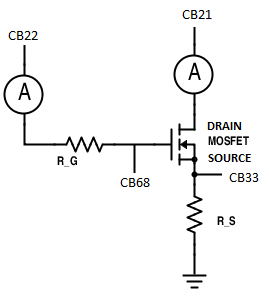
\includegraphics[scale=.5]{mosfet}
\caption{Schema del circuito montato sulla breadboard.}
\label{fig:circ}
\end{figure}

Dal momento che la scheda di acquisizione può erogare al massimo 10 mA e 10 V, abbiamo dovuto dimensionare $R_S$ in modo tale che nelle condizioni estreme, quindi $V_{GS} = V_{DS} = 10 V$, la corrente non raggiungesse i 10 mA. Per R = 1.025 $\pm$ 0.8 $\%$ k$\Omega$ si ha che la corrente massima che può circolare nel circuito, misurata tramite l'amperometro collegato in serie alla CB21, non raggiunge 8 mA, per cui abbiamo preso questo valore della resistenza per $R_S$. Nelle varie prove effettuate è stato impiegato un altro amperometro collegato in serie alla CB22 per misurare la corrente che circola verso il GATE. Ciò che è risultato è che pur avendo impostato il fondoscala più basso la corrente si manteneva costantemente sotto soglia. Questo significa che nel seguito è possibile considerare con ottima approssimazione uguali le correnti al DRAIN e al SOURCE. Inoltre, visto che non si sono praticamente rilevate correnti, la resistenza $R_G$ che noi abbiamo inizialmente scelto di 1 k$\Omega$ non influenza sostanzialmente il circuito.\\
Tramite il VI \texttt{Vin$\_$Vout$\_$2C} abbiamo impostato diversi valori delle tensioni al GAIN e al DRAIN, con il vincolo $V_{GS} = V_{DS}$, cercando il valore della tensione di soglia, ovvero il valore per cui la corrente al DRAIN fosse 1 mA. Abbiamo trovato $V_{GS(th)}$ = 2.23 $\pm$ 0.02 V, simile al valore tipico dichiarato dal datasheet.

\section{Corrente di DRAIN vs tensione sul GATE}

Per misurare come la corrente di DRAIN dipenda dalla tensione di GATE abbiamo utilizzato il VI \texttt{FET$\_$vs$\_$GATE} che fissa il valore della tensione al DRAIN e spazza un intervallo di tensioni da impostare per il GATE. Come prima misura abbiamo impostato $V_{DS}$ = 3 V e spazzato un intervallo di tensioni da 1 V a 7 V. I dati sperimentali sono rappresentati in figura \ref{fig:es4_3}. Come si vede l'andamento non è lineare, inoltre la tensione $V_S$ satura quando $V_S$ si avvicina ai 3 V. Questo perché la tensione al SOURCE deve mantenersi costantemente inferiore alla tensione al DRAIN, quindi per quanto si aumenti la tensione al GATE, non si potrà far scorrere una corrente per cui $V_S \geq V_{DS}$. 

\begin{figure}[htp]
\centering
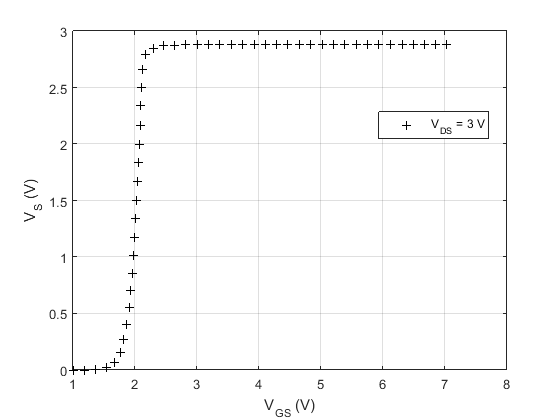
\includegraphics[scale=.5]{es4_3}
\caption{Grafico $V_S$ vs $V_{GS}$ per $V_{DS}$ = 3 V.}
\label{fig:es4_3}
\end{figure}

Fin qui si è assunto che la corrente che scorre al SOURCE sia uguale a quella al GATE. Difatti questa ipotesi è stata già precedentemente verificata, collegando l'amperometro al GATE. Un altro modo per verificare la validità dell'ipotesi é collegare l'amperometro in serie al DRAIN e verificare che la corrente misurata sia compatibile con quella calcolata misurando la tensione al SOURCE. Abbiamo effettuato due prove, in tabella \ref{tab:es6} sono riportati i risultati. Come si vede i valori delle due correnti sono compatibili fra loro.

\begin{table}[htp]
\centering
\caption{Verifica che $I_S = I_D$.}
\label{tab:es6}
\begin{tabular}{|c|c|c|c|c|}
\hline 
$V_{GS}$ (V)& $V_{DS}$ (V) & $V_S$ (V) & $I_D$ (mA)& $I_S$ (mA) \\ 
\hline 
5 & 5 & 2.8875(2) & 2.81 $\pm$ 0.8 $\%$ & 2.82(2) \\ 
\hline 
6 & 6 & 3.849(1) & 3.70 $\pm$ 0.8 $\%$ & 3.76 $\pm$ 0.03 \\ 
\hline 
\end{tabular} 
\end{table}

Abbiamo ripetuto la misura fatta con il VI \texttt{FET$\_$vs$\_$GATE} variando il valore di $V_{GS}$. I vari grafici ottenuti sono riportati in figura \ref{fig:all}. Si vede chiaramente come i grafici hanno tutti lo stesso andamento a basse tensioni al punto che si sovrappongono, mentre saturano ciascuno corrispondentemente al valore di $V_{DS}$, a parte per i casi $V_{DS}$ = 9, 10 V in cui non sono state raggiunte tensioni sufficienti per osservare la saturazione.\\

\begin{figure}[htp]
\centering
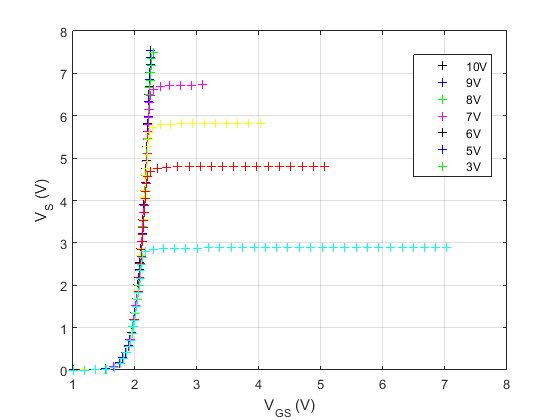
\includegraphics[scale=.5]{all}
\caption{Grafico $V_S$ vs $V_{GS}$ per vari valori di $V_{GS}$.}
\label{fig:all}
\end{figure}

Per ottenere una stima della transconduttanza abbiamo preso i dati relativi al caso $V_{DS}$ = 10 V, escludendo i primi 10 dati in quanto corrispondenti alla regione di interdizione del transistor. L'andamento previsto è di tipo quadratico, precisamente:

\begin{equation}
I = I_0 \, (V-V_T)^2
\end{equation}

dove $V_T$ è la tensione di soglia del MOSFET. Il grafico del fit è riportato in figura \ref{fig:fit}.

\begin{figure}[htp]
\centering
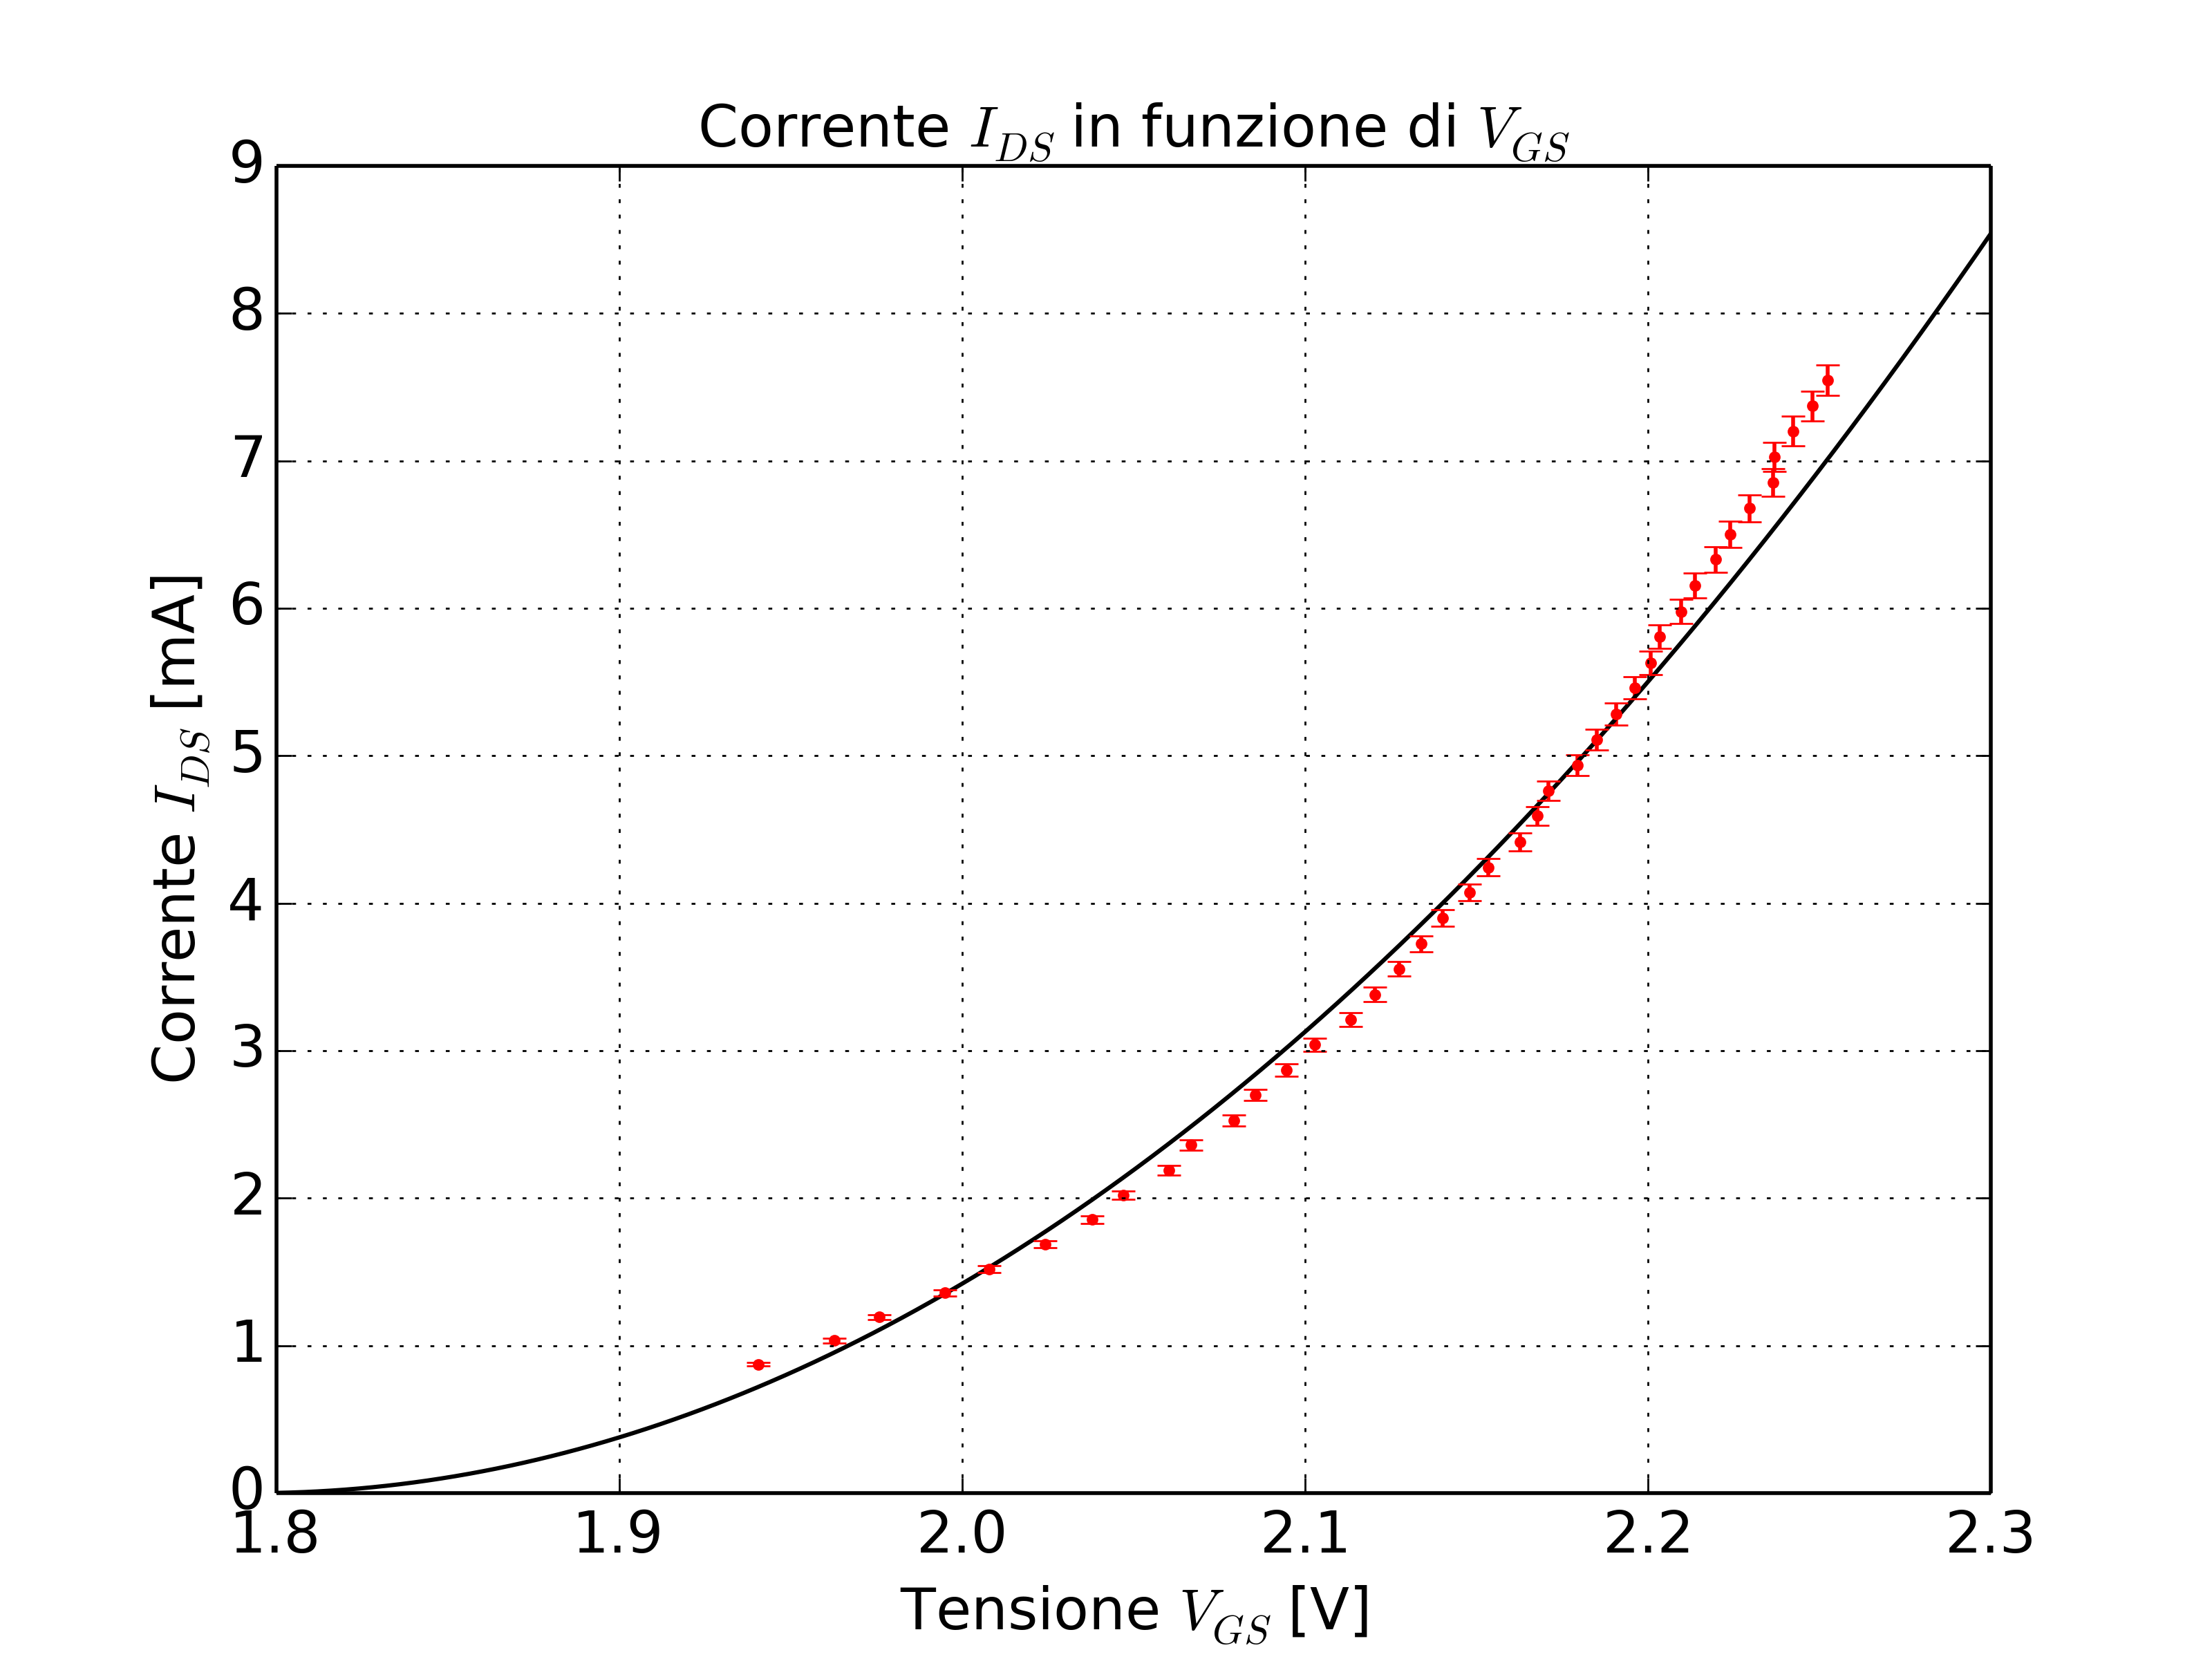
\includegraphics[scale=.4]{fit_es8}
\caption{Fit quadratico di $V_{GS} \, vs \, I_{DS}$.}
\label{fig:fit}
\end{figure}

I risultati sono stati $I_0 = 33(1)$ mA, $V_T = 1.793(5)$ V. Estrapolando il grafico fino a 10 V si ottiene una stima della transconduttanza, pari a 224(7) mS (figura \ref{fig:fit2}), significativamente più piccolo del valore indicato sul datasheet (valore tipico 320 mS).

\begin{figure}[htp]
\centering
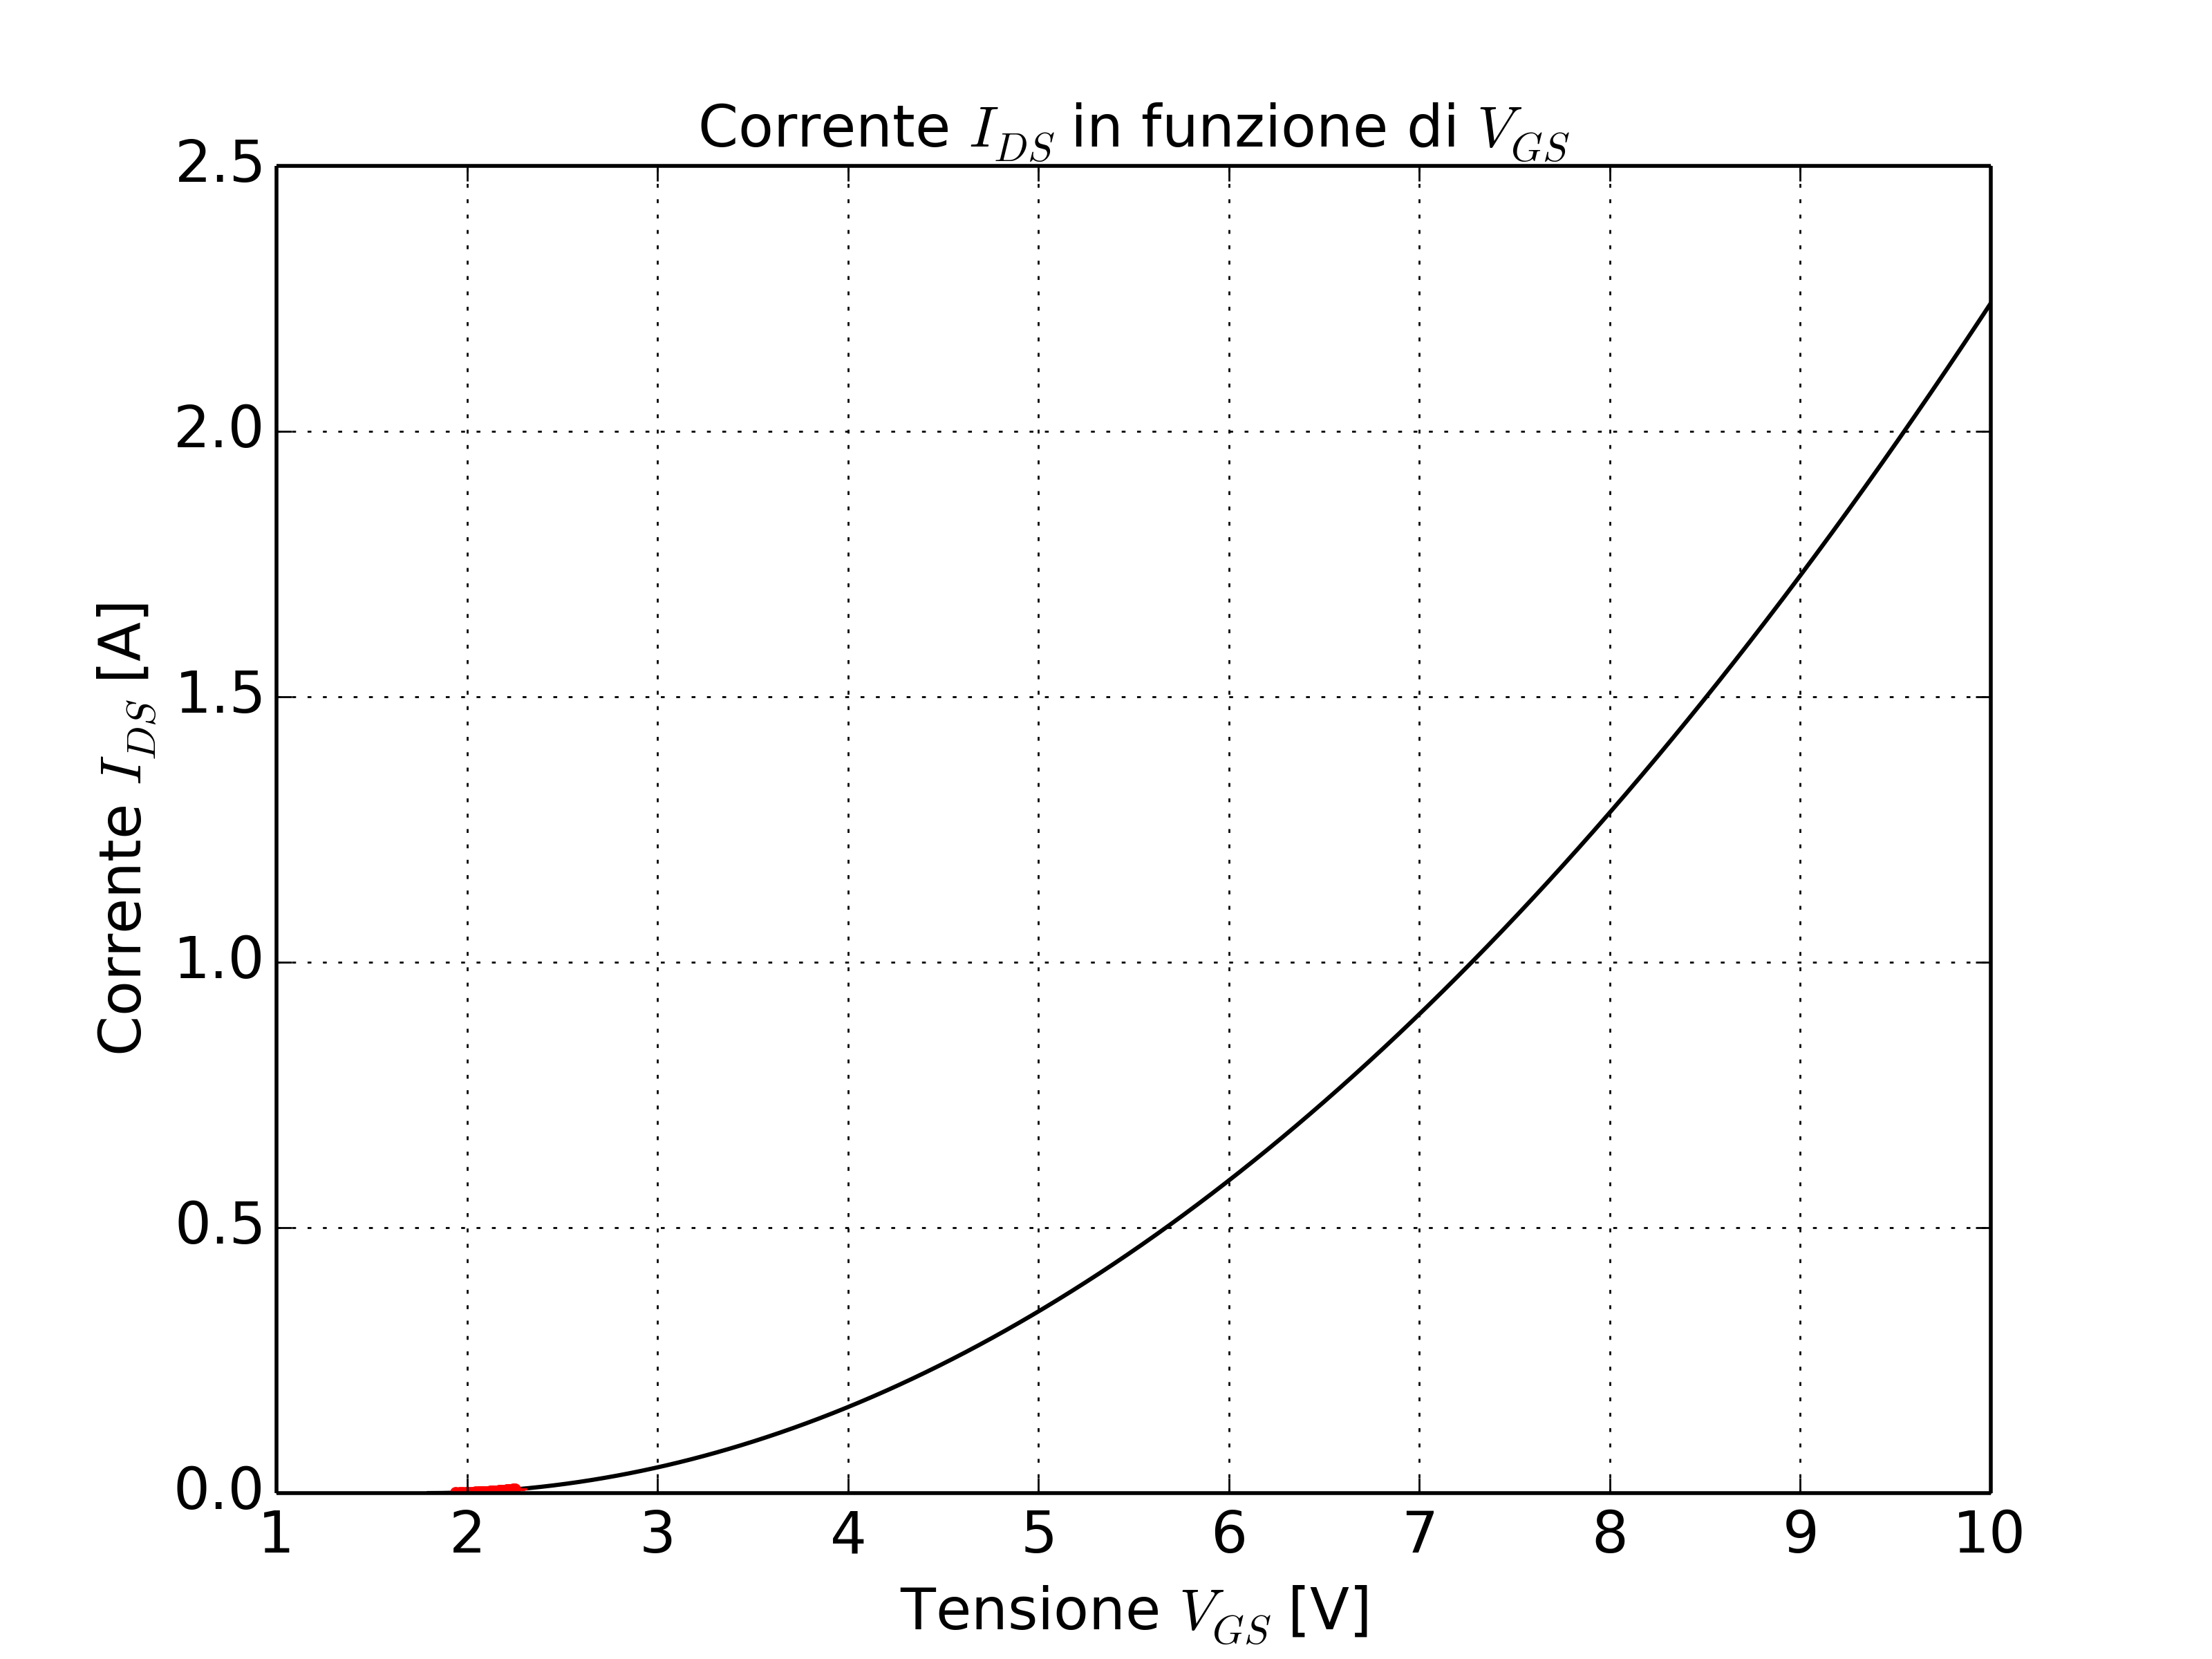
\includegraphics[scale=.4]{fit_es8_es}
\caption{Estrapolazione fino a $V_{DS}$ = 10 V del grafico del fit \ref{fig:fit}}
\label{fig:fit2}
\end{figure}

\section{Corrente di drain vs tensione di drain}
Proviamo ora a visualizzare l'andamento della corrente di drain $I_{DS}$ in funzione della tensione di drain $V_{DS}$. Sappiamo che i \textsc{mosfet} sono degli ottimi esempi di componenti a transconduttanza, vale a dire la capacità di mantere costante la corrente, fissata una certa tensione di \textit{gate} $V_{GS}$. Questo comportamento si evidenzia in particolar modo per tensioni di drain superiori alla tensione di soglia $V_T$, nella cosiddetta zona di saturazione. Si veda il grafico tratto dall'Horowitz e riportato in Figura (\ref{fig:horo-linear_saturation}). Fissando dei valori della tensione di gate $V_{GS} = 2, 3, 4 \si{V}$, abbiamo cercato di visualizzare la regione lineare esplorando un intervallo opportuno di tensioni $V_{DS}$. La scelta di $V_{GS} = 2$V è la più infelice delle tre, poichè sappiamo che la regione lineare si estende fino a un valore $V_{DS(sat)} = V_{GS} - V_T$, e si è stimato negli esercizi precedenti che per il nostro \textsc{mosfet} vale $V_T \simeq 2.2 V$, per cui nelle tensioni positive di drain non dovremmo mai trovarci nella zona lineare.\\ 

\begin{figure}
\centering
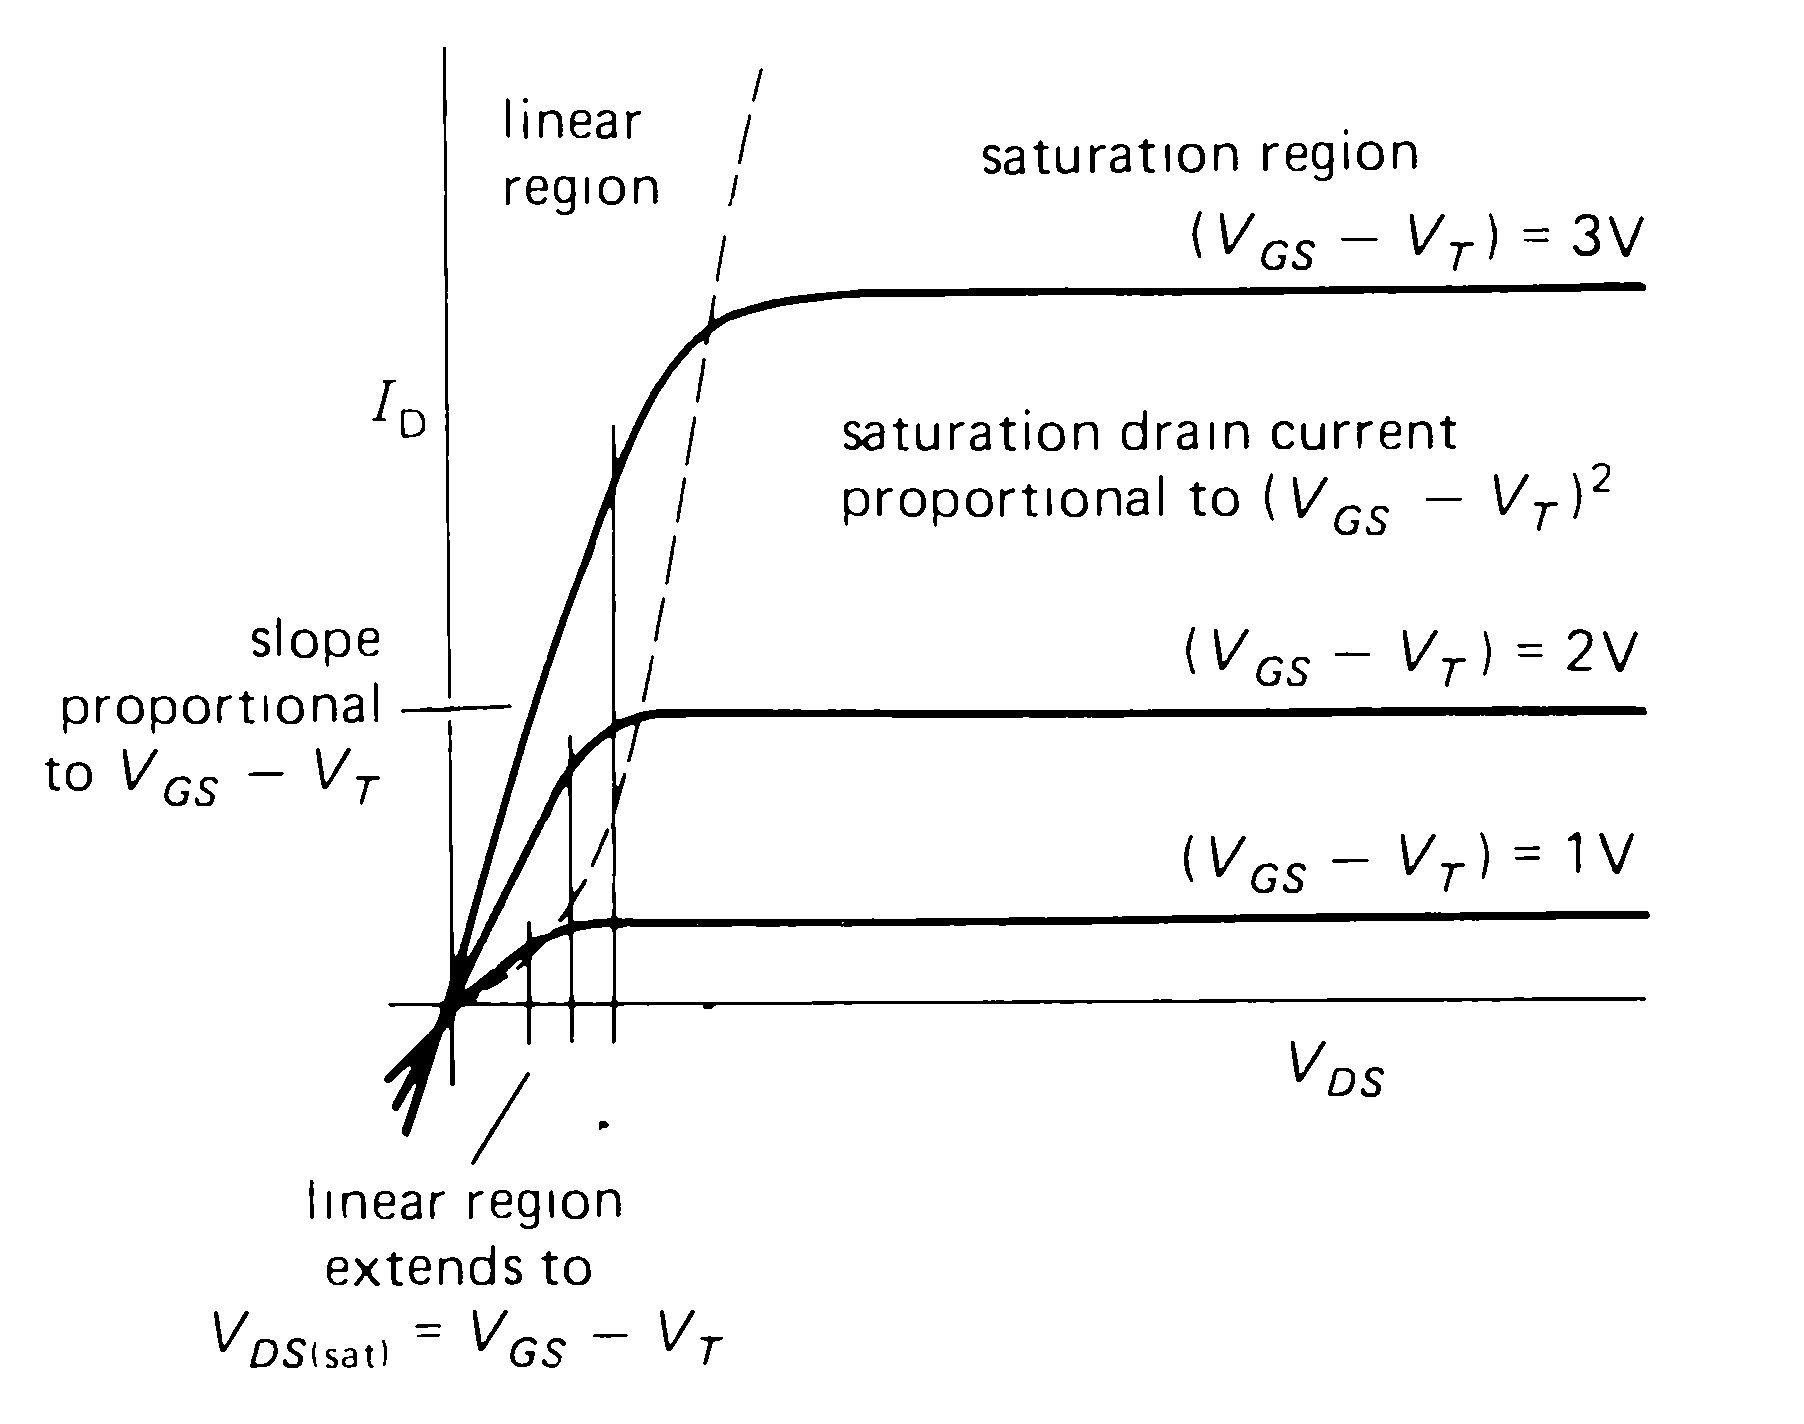
\includegraphics[width=0.9\linewidth]{./horo-linear_saturation}
\caption{Andamento di $I_{DS}$ in funzione di $V_{DS}$ per dati valori di tensione di gate.}
\label{fig:horo-linear_saturation}
\end{figure}

In ogni caso, esaminando i dati acquisiti nelle Figure (\ref{fig:es9_prova_vg3}, \ref{fig:es9_prova_vg4}), nonostante il comportamento lineare sia facilmente intuibile, notiamo un evidente problema nel processo di acquisizione: durante tutta la spazzata sulle tensioni i valori delle correnti (che si ottengono moltiplicando il segnale della \textsc{cb33} per il valore della resistenza sul \textit{source}) sembrano dei "gradini" che mal si adattano ad una funzione continua. Riteniamo che questo possa essere dovuto ad una limitazione del campionamento della nostra scheda di acquisizione \textsc{pci6024e} (che acquisisce a 200kS/s), ipotesi supportata dal fatto che si è notato un comportamento analogo su tutti i tavoli con lo stesso modello di scheda. In Figura (\ref{fig:es9_multivg}) si riporta un multiplot riassuntivo. Data la scarsa qualità dei dati, ha poco senso calcolare esplicitamente la relazione fra $V_{GS}$ e pendenza della retta nella regione lineare (è noto che la \textit{slope} $ \propto V_{GS} - V_T$ ); annotiamo tuttavia un aumento della pendenza al crescere della tensione di gate.\\

\begin{figure}
\centering
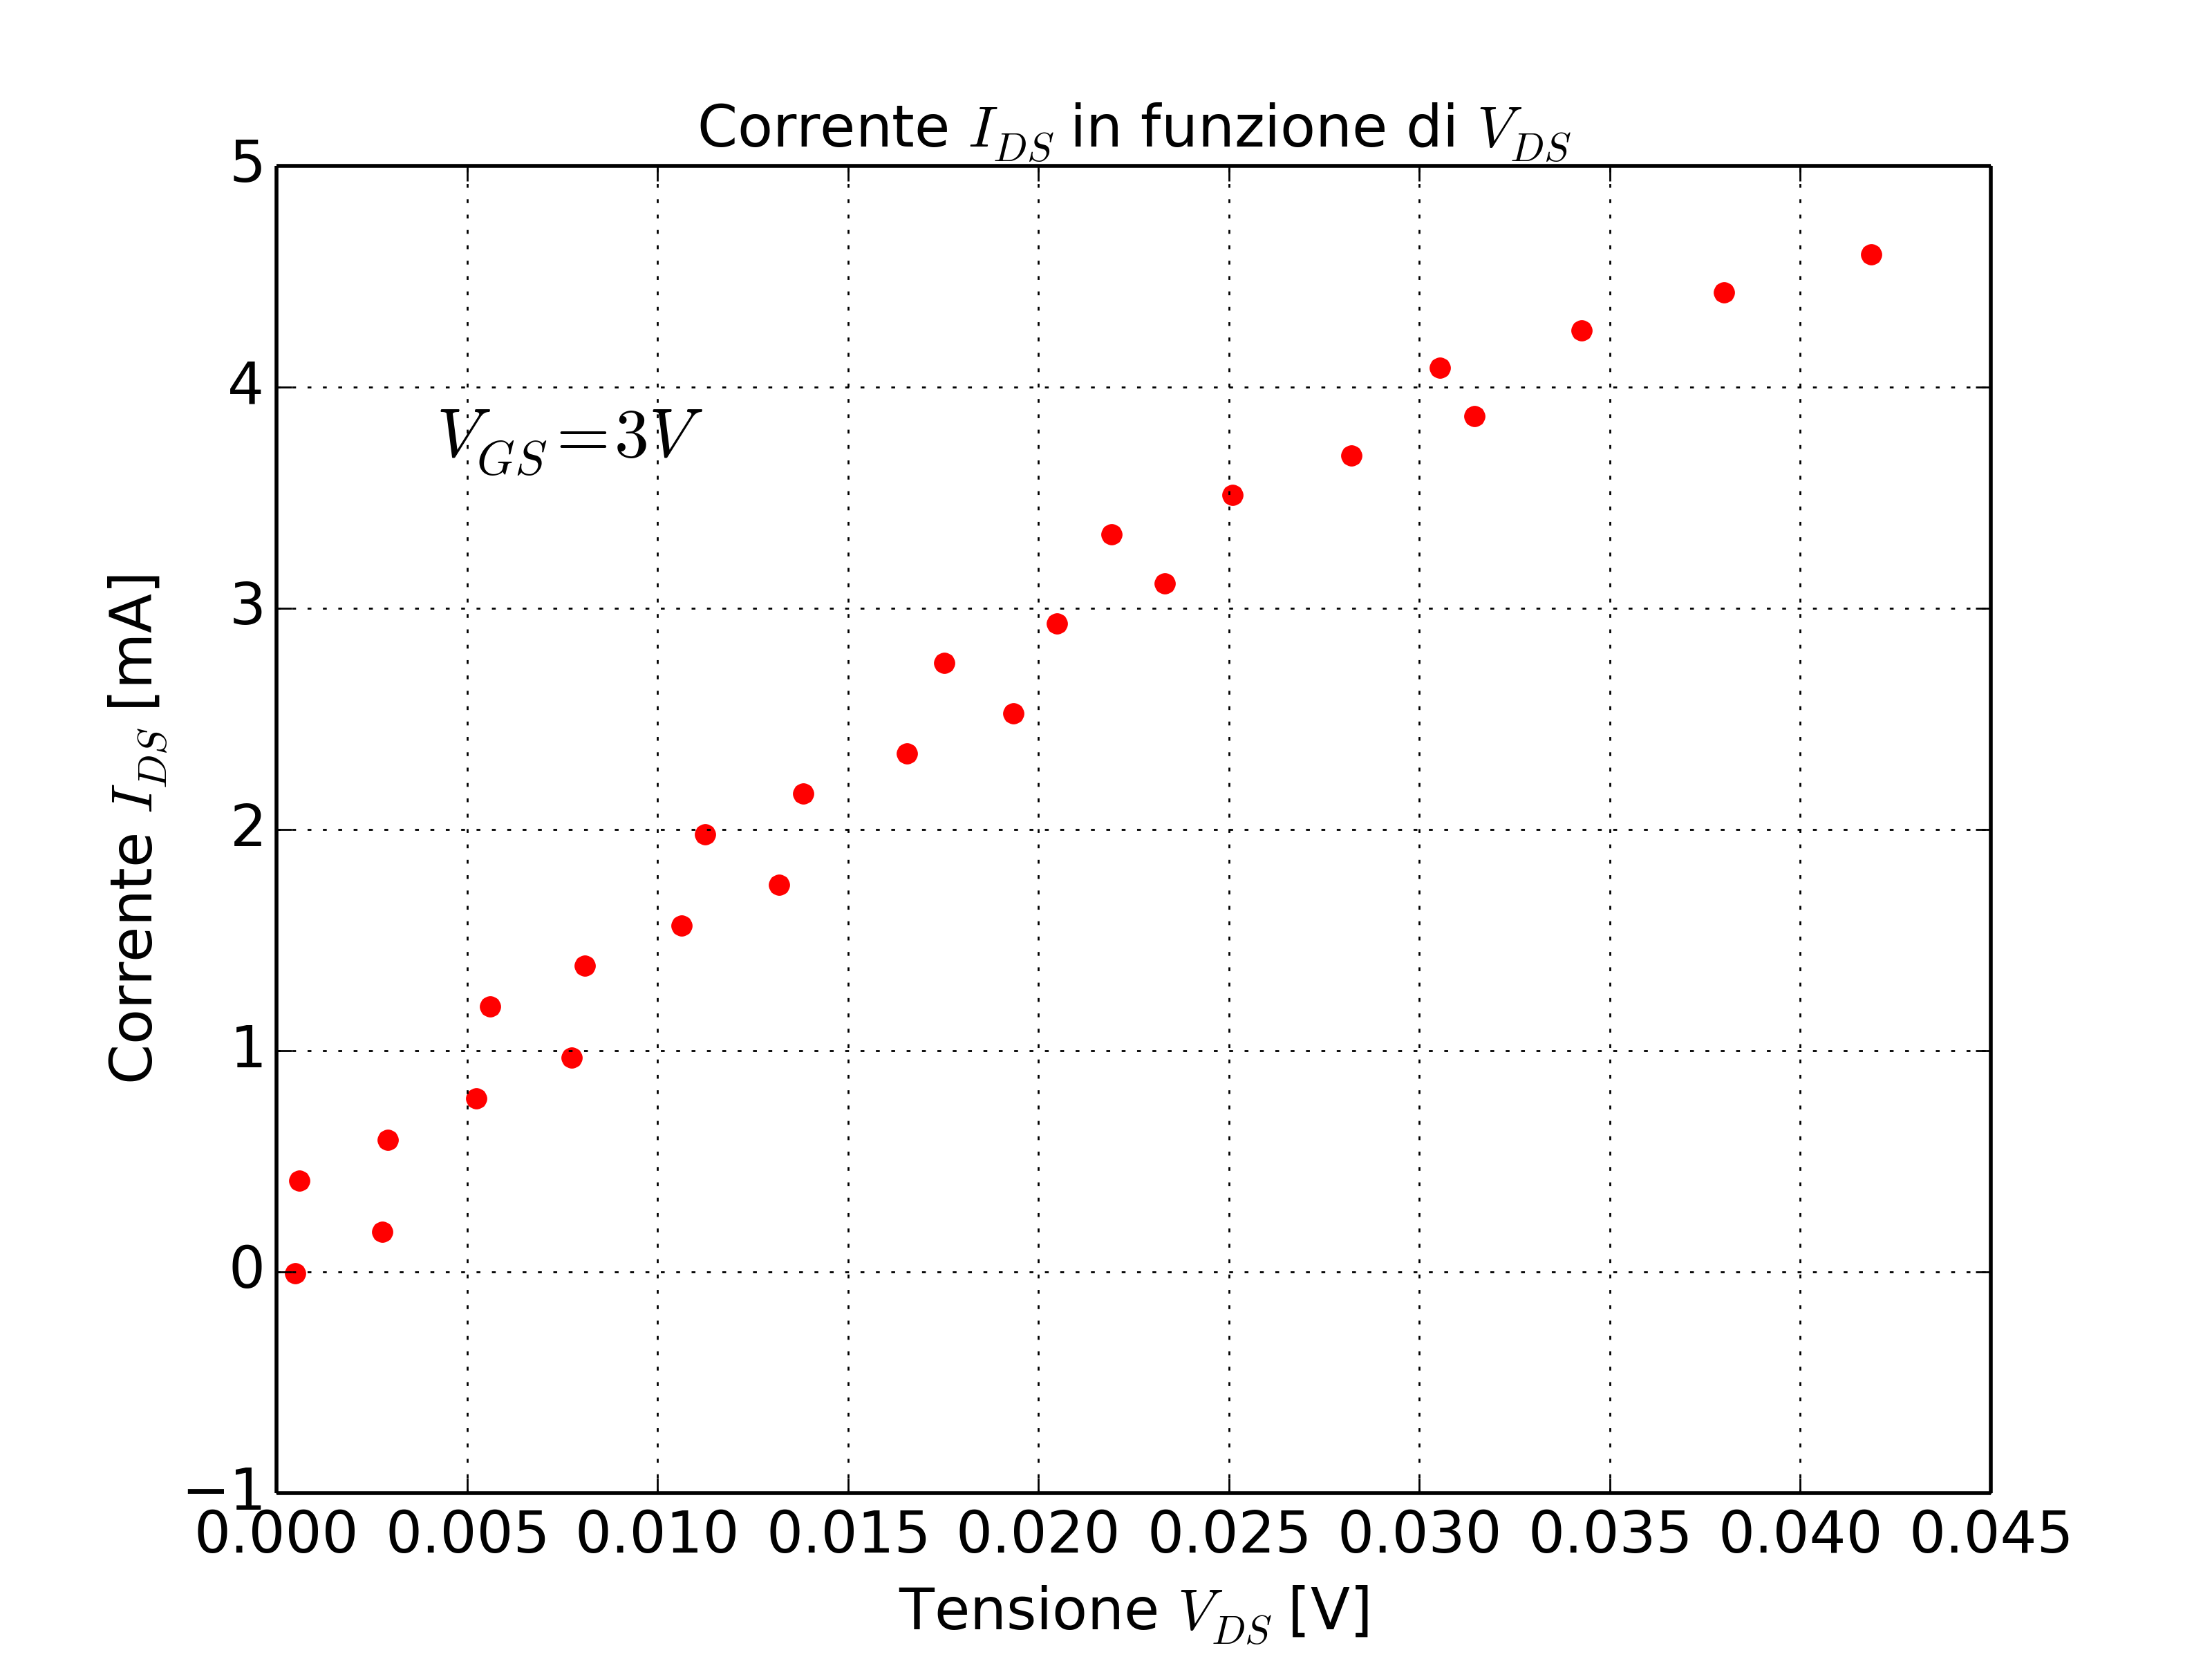
\includegraphics[width=0.8\linewidth]{./es9_prova_vg3}
\caption{$I_{DS}$ vs $V_{DS}$ per fissata tensione di gate = 3V.}
\label{fig:es9_prova_vg3}
\end{figure}

\begin{figure}
\centering
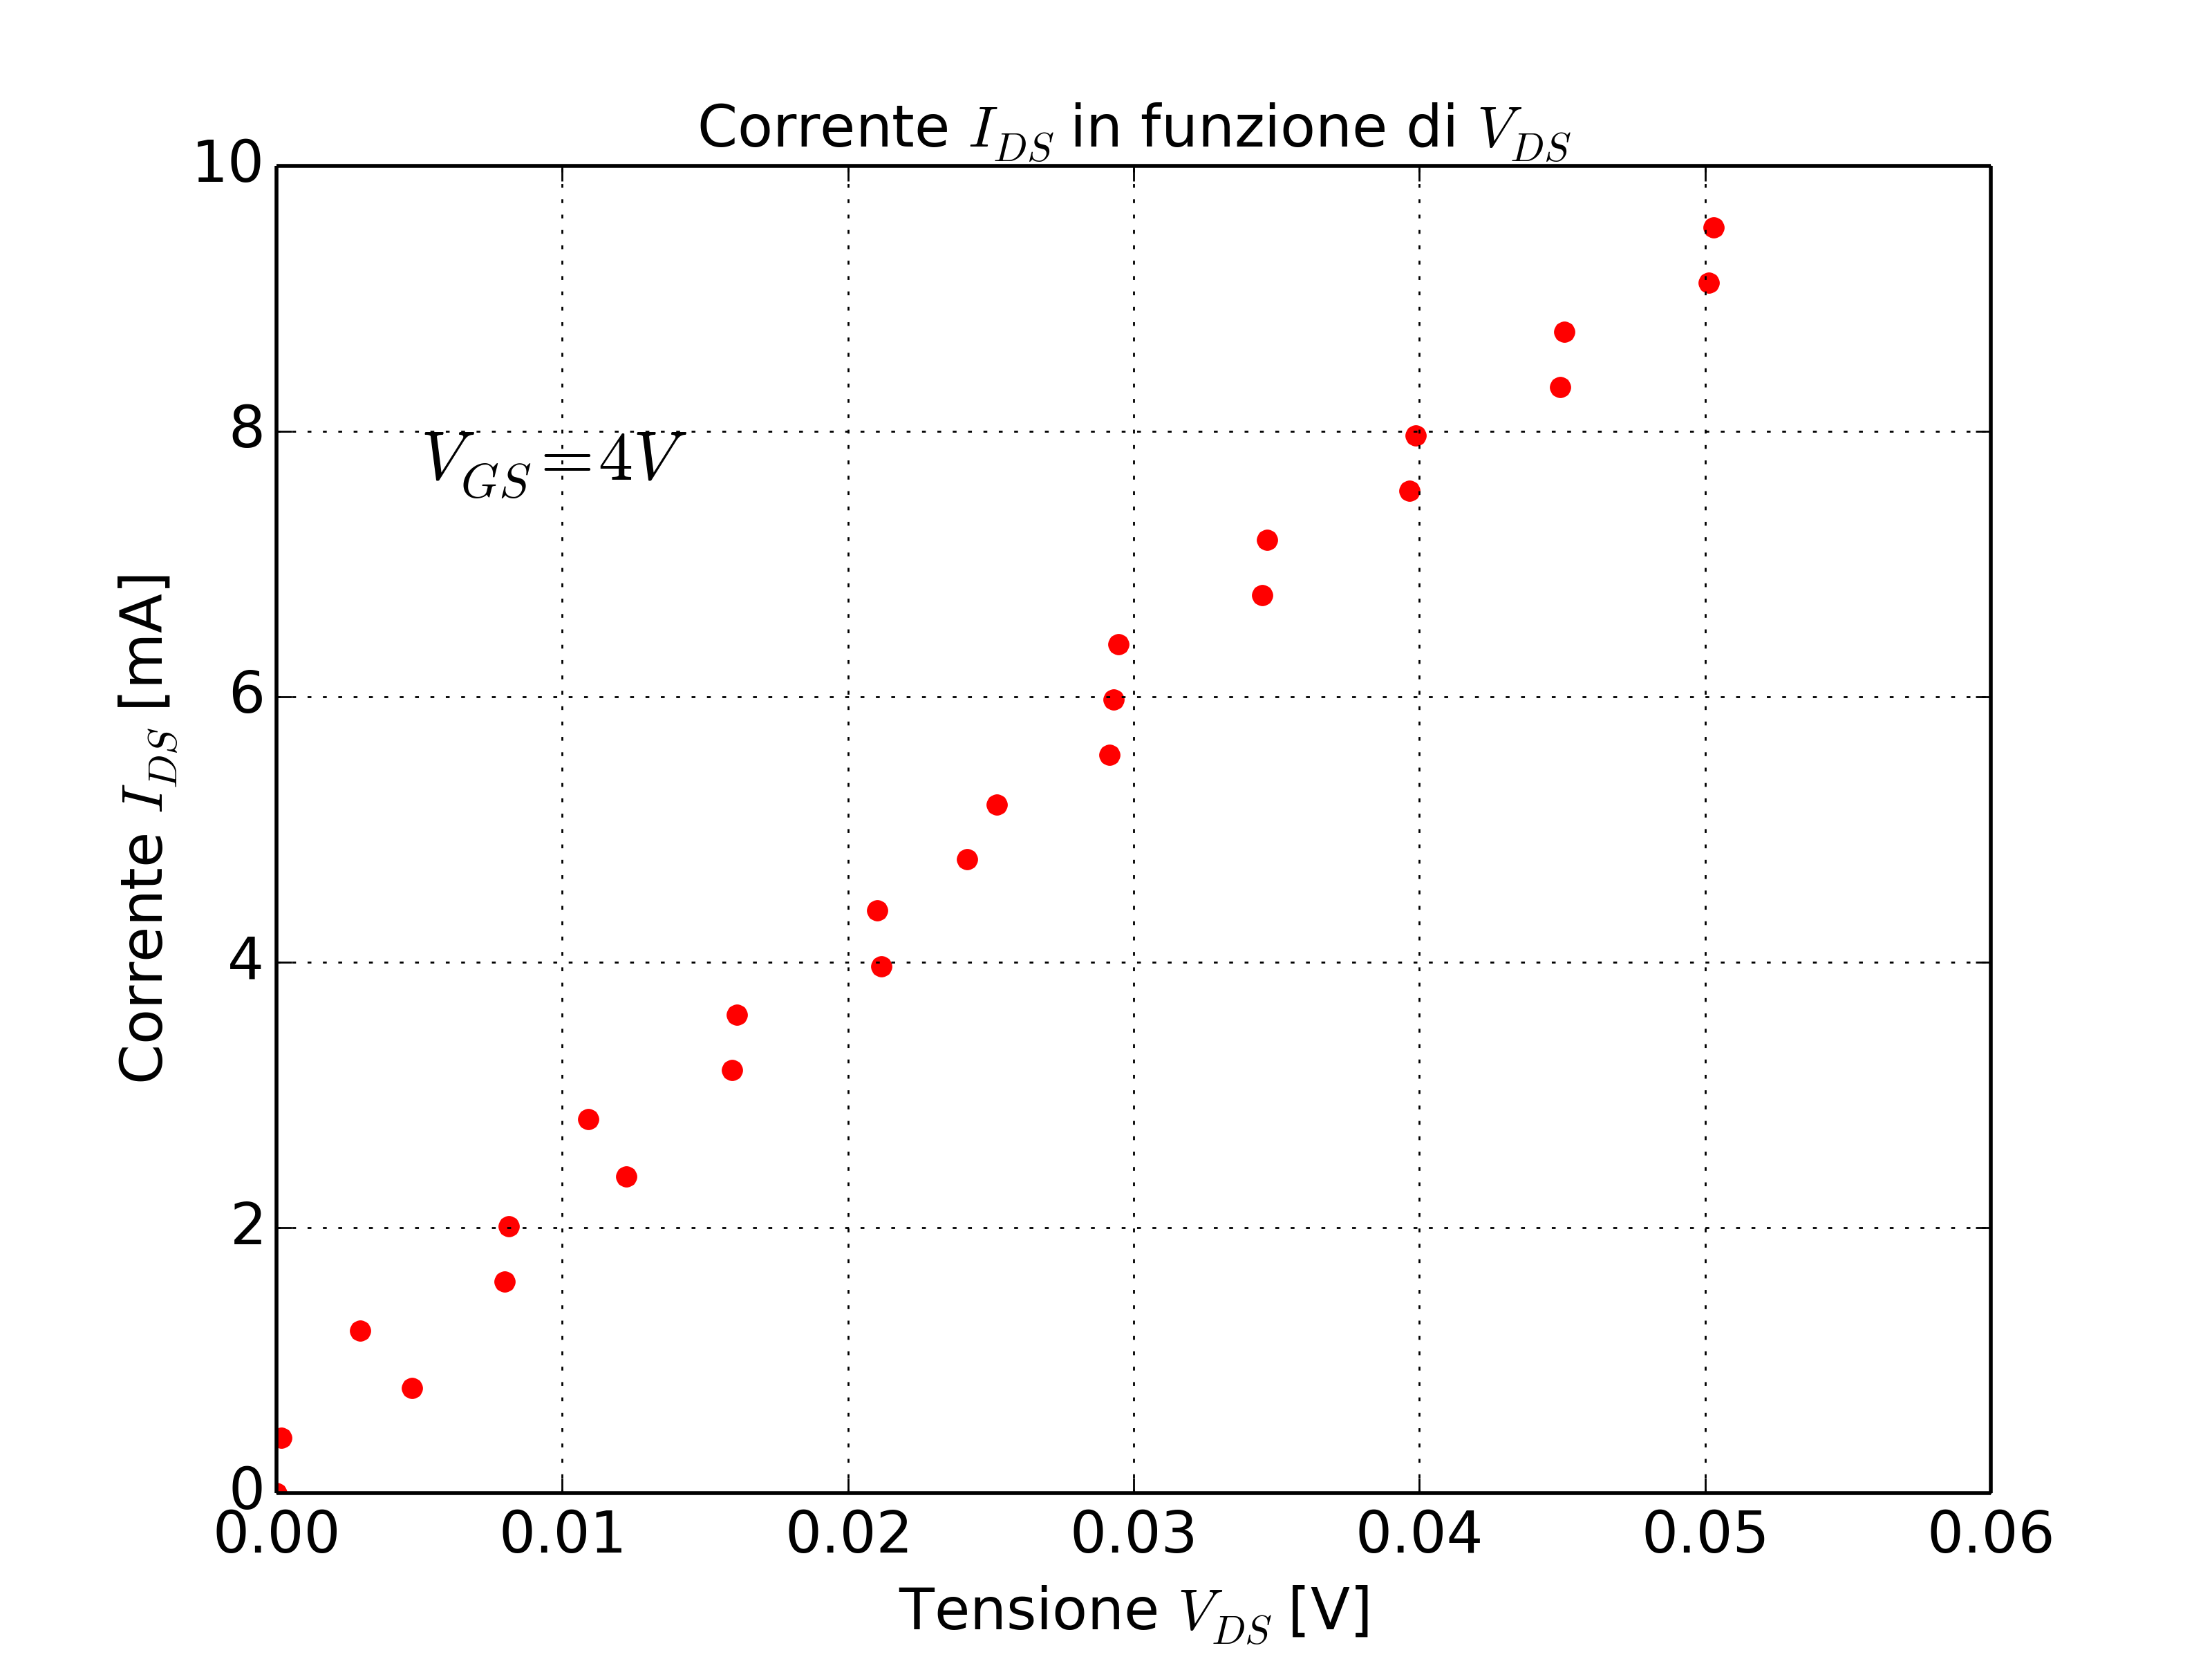
\includegraphics[width=0.8\linewidth]{./es9_prova_vg4}
\caption{$I_{DS}$ vs $V_{DS}$ per fissata tensione di gate = 4V.}
\label{fig:es9_prova_vg4}
\end{figure}

\begin{figure}
\centering
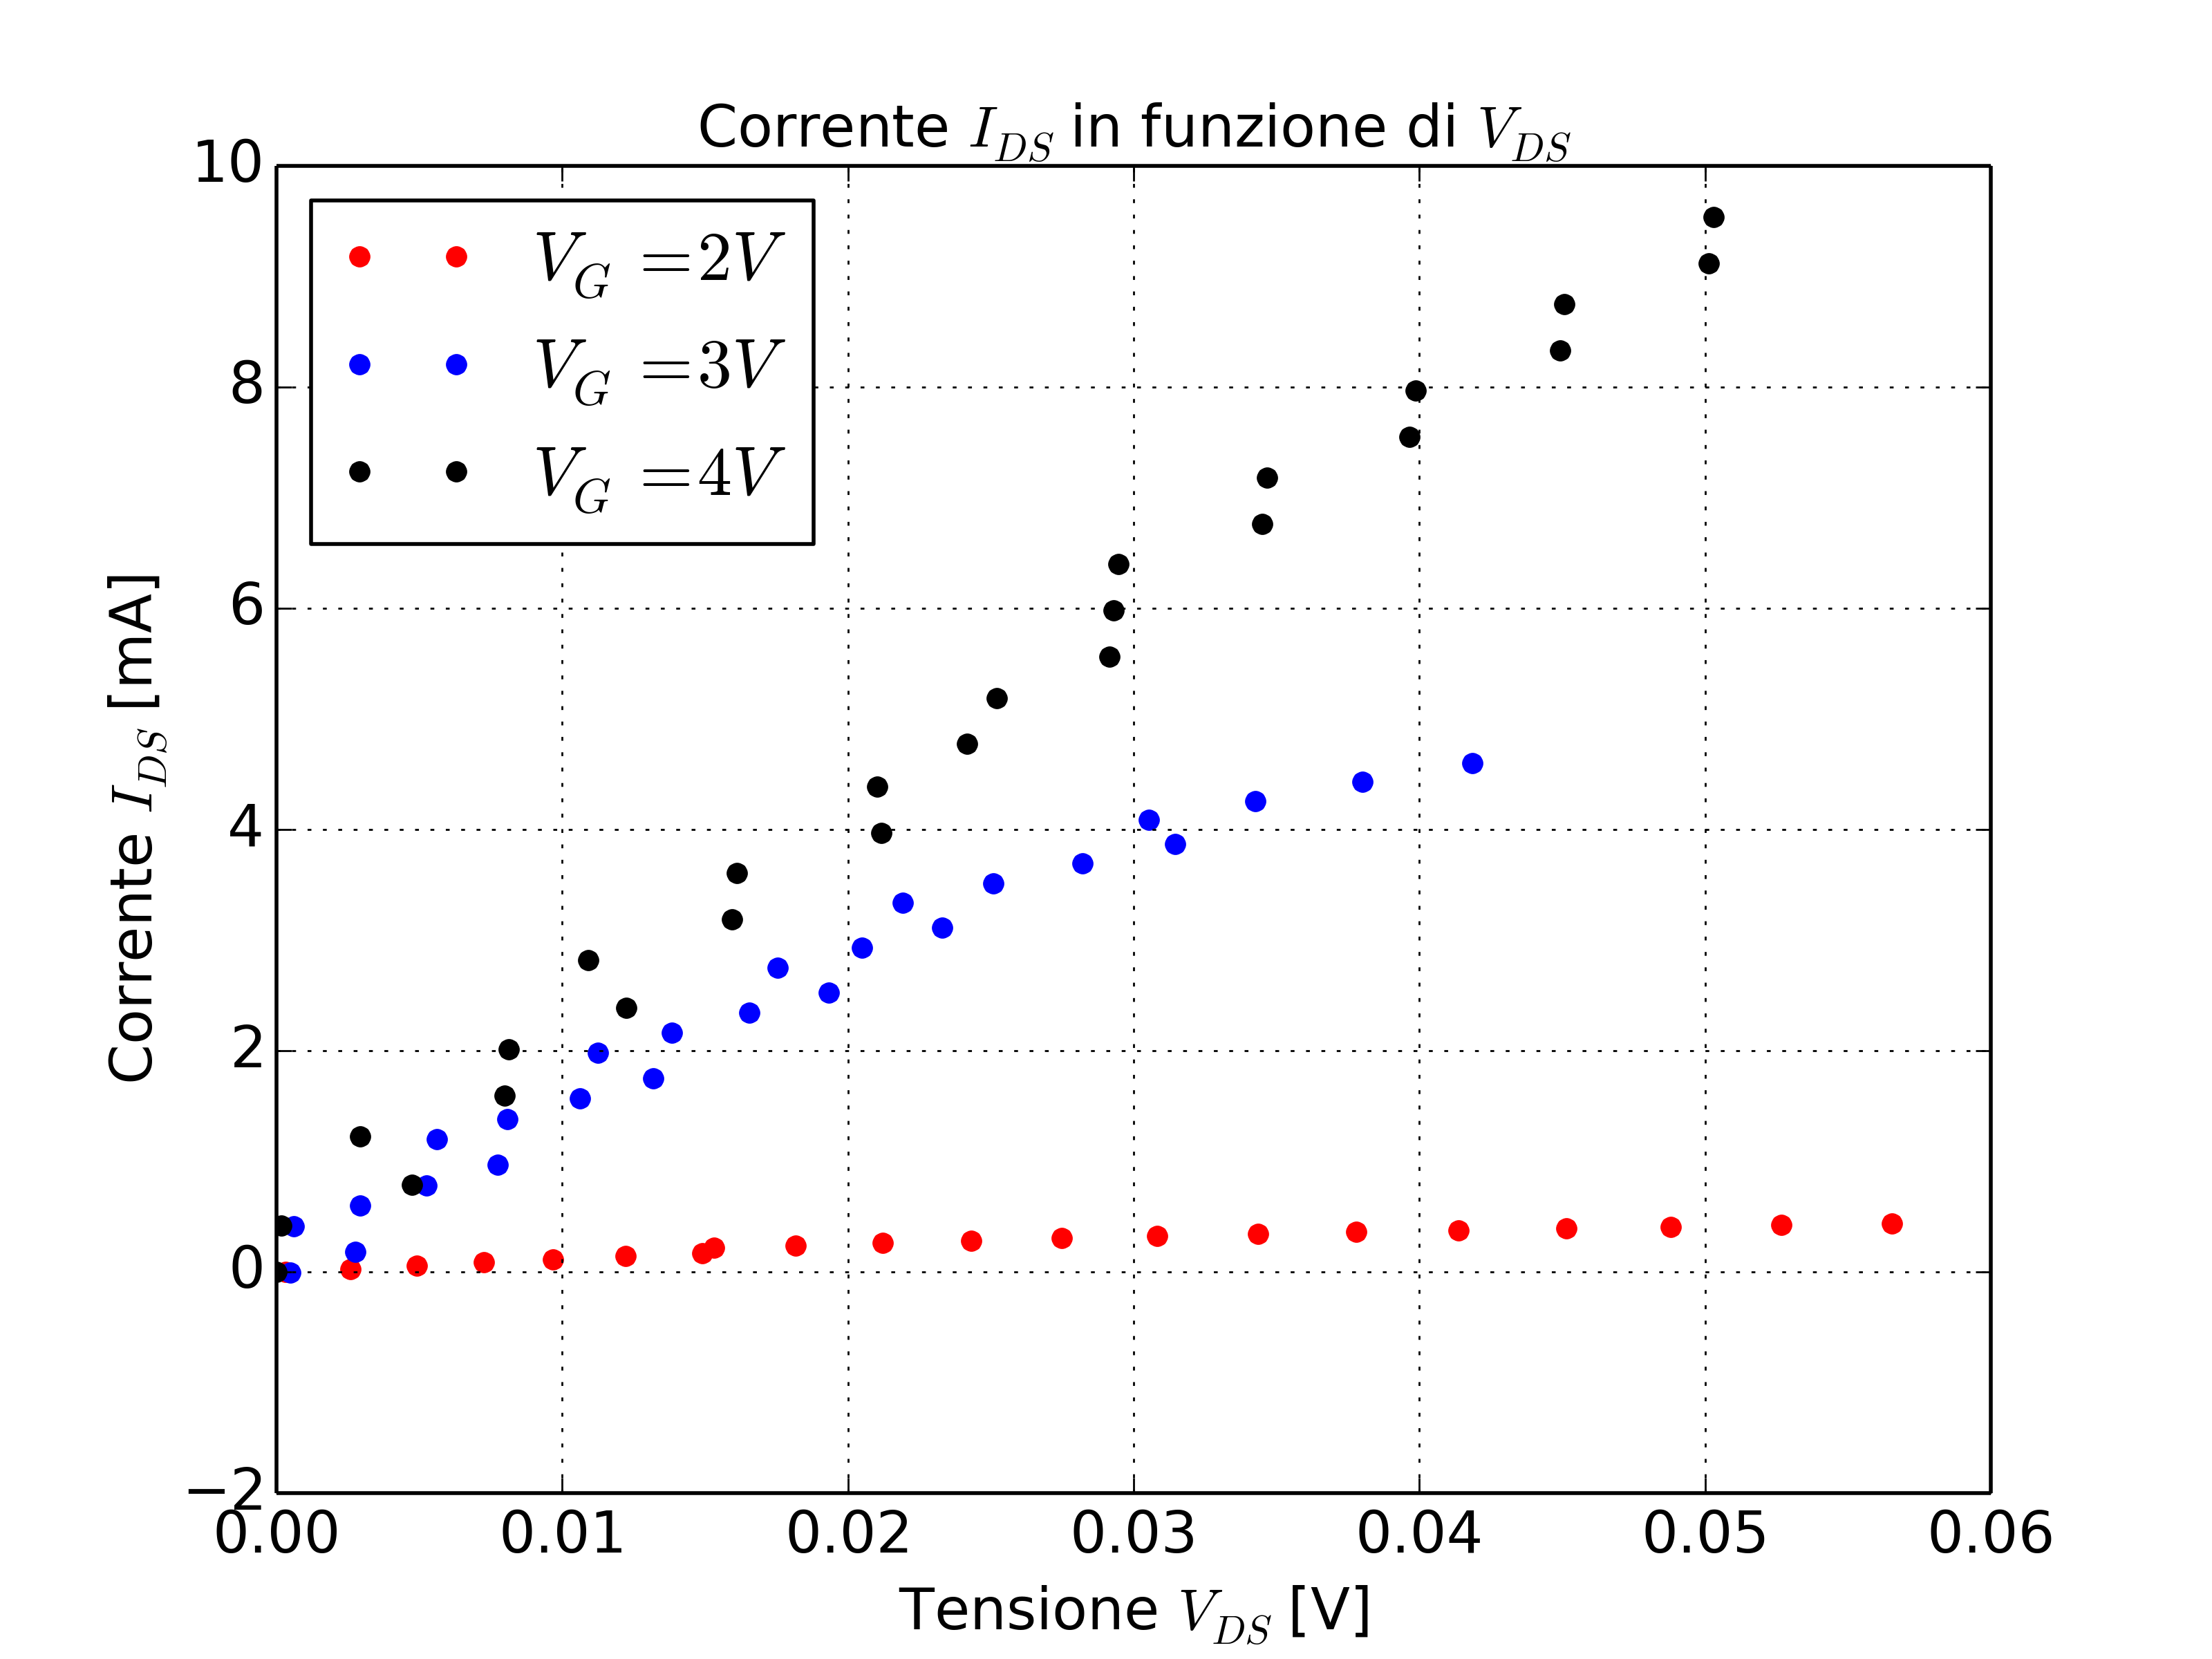
\includegraphics[width=0.9\linewidth]{./es9_multivg}
\caption{Multiplot $I_{DS}$ vs $V_{DS}$ per tensioni di gate = 2, 3, 4V.}
\label{fig:es9_multivg}
\end{figure}

Proviamo ora ad acquisire qualche dato nella regione di saturazione: questa volta la DAQ sembra non avere particolari problemi e, come si vede in Figura (\ref{fig:es11_multivg}), la corrente rimane praticamente costante su intervalli di diversi volt di tensione di drain. Il grafico è in scala logaritmica sulle y per questioni di scala fra le due serie di punti riportate. \\

\begin{figure}
\centering
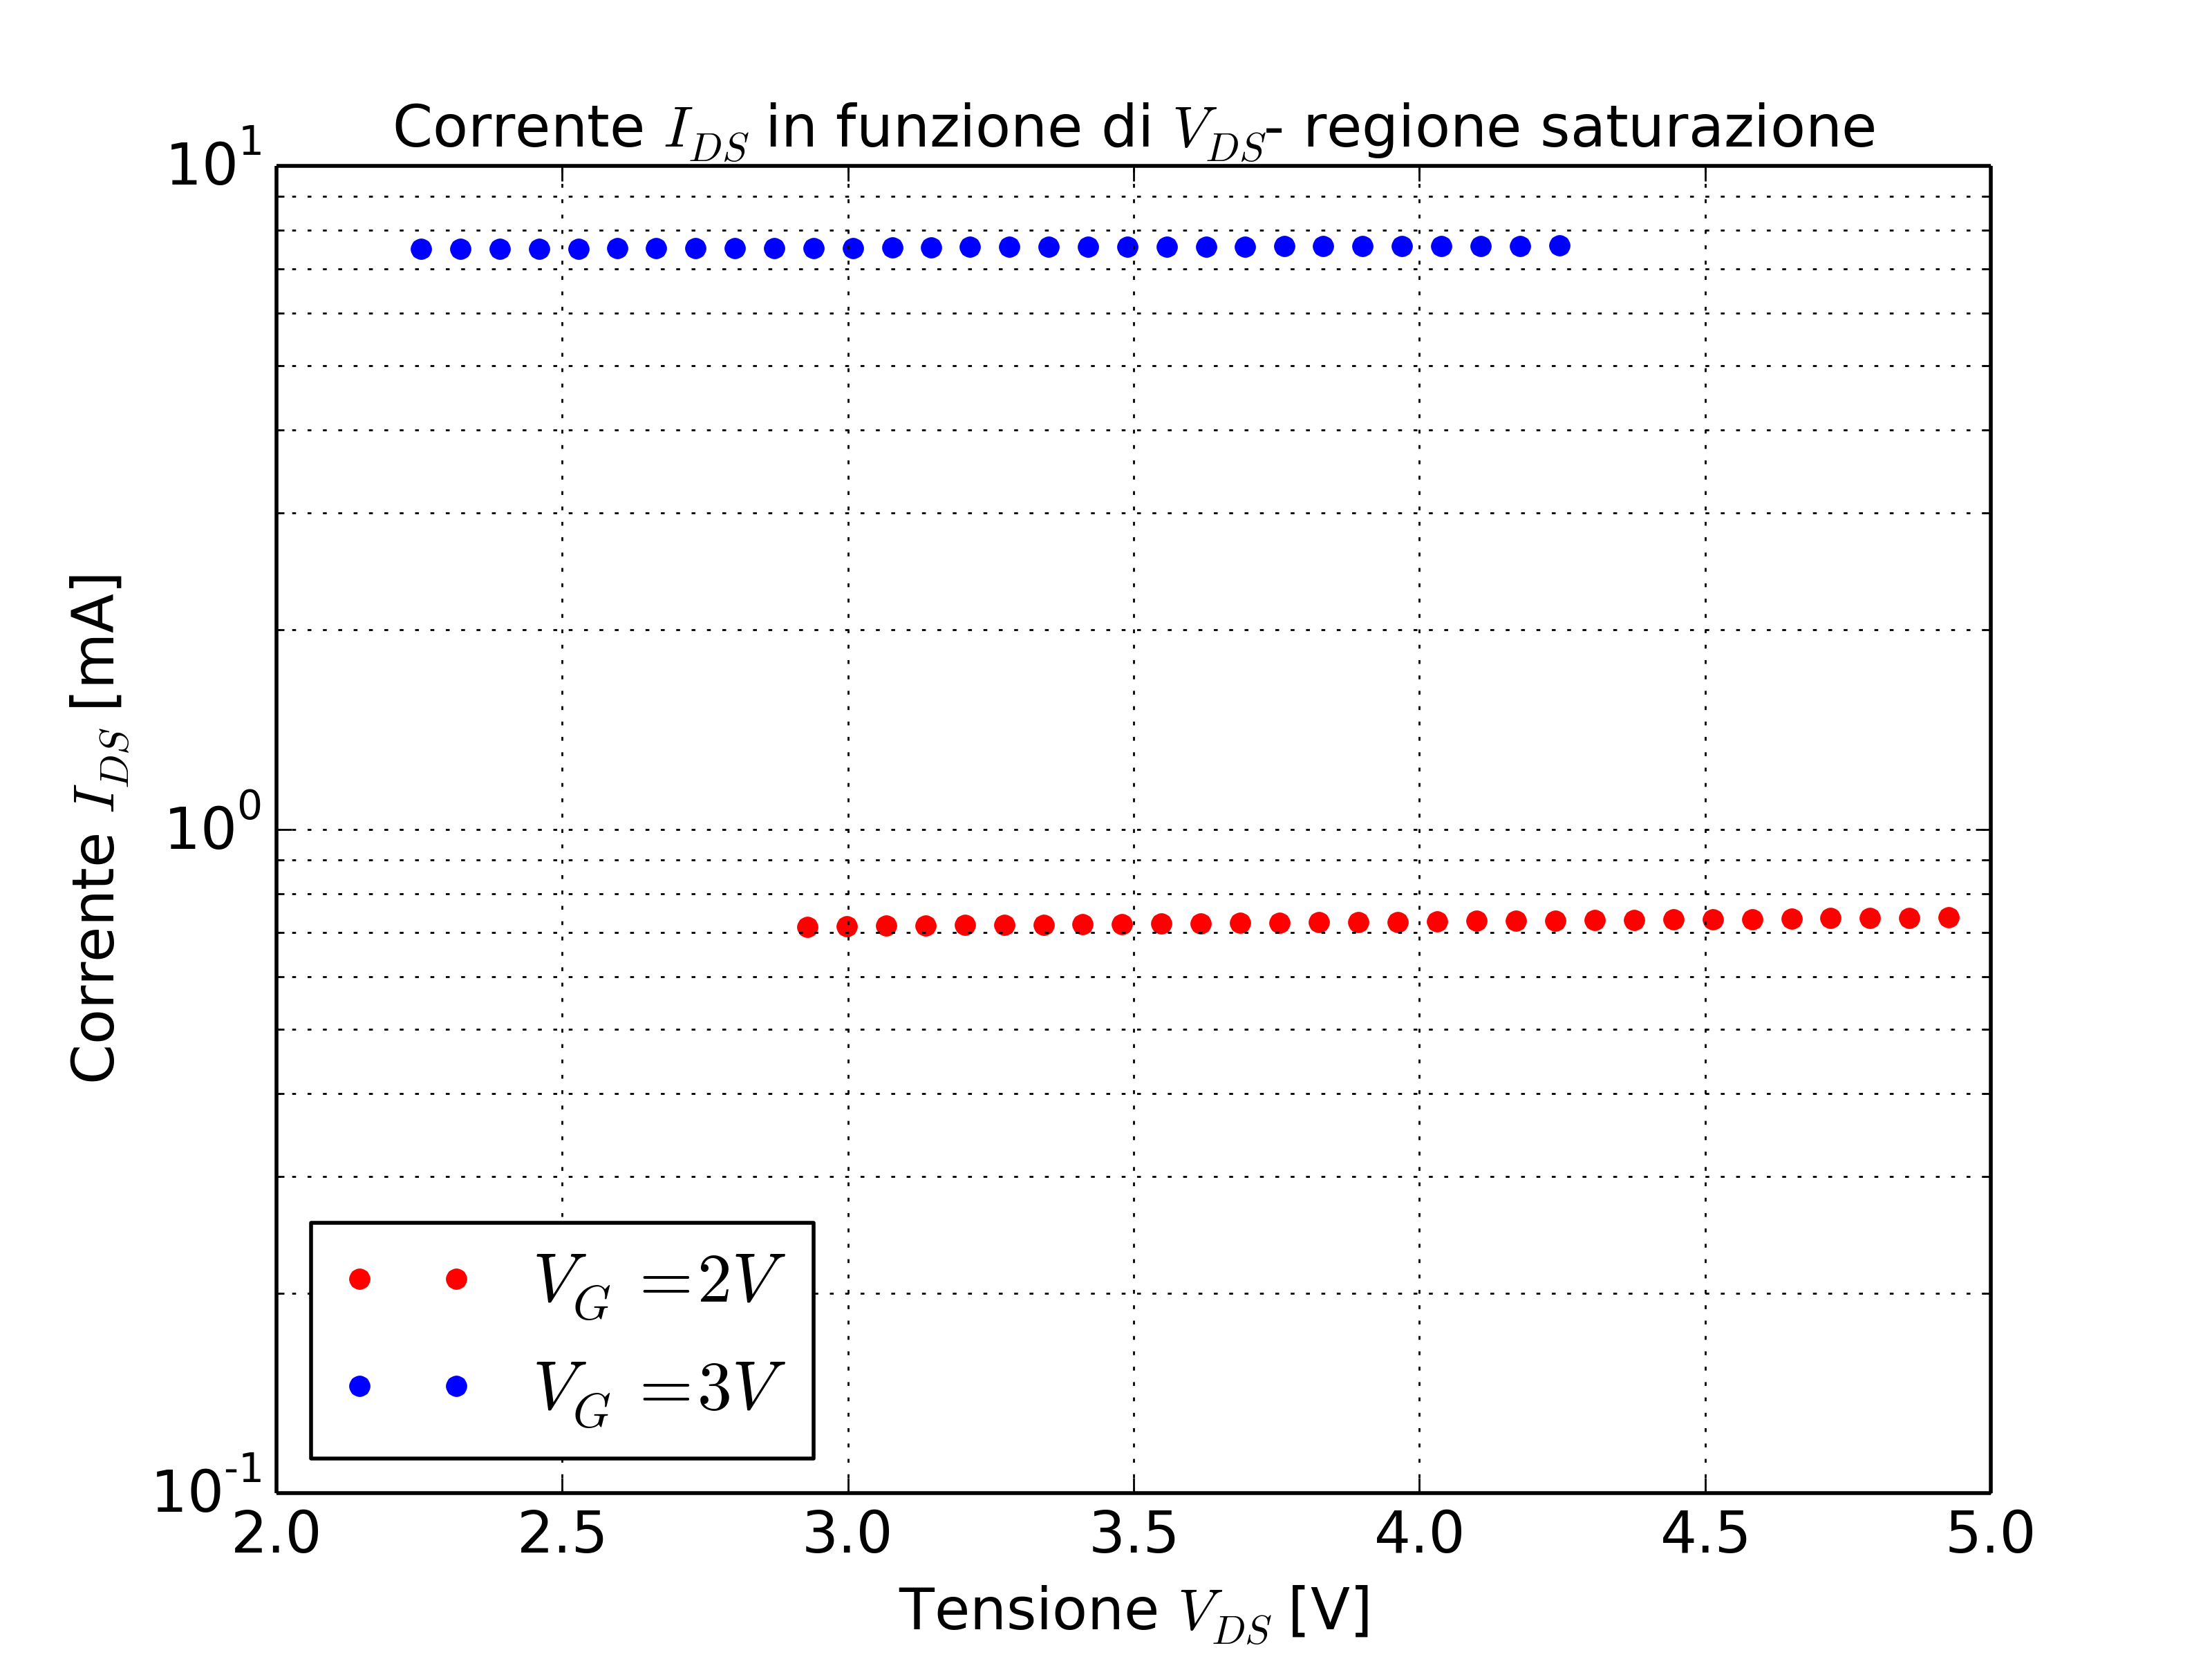
\includegraphics[width=0.9\linewidth]{./es11_multivg}
\caption{Regione di saturazione $I_{DS} vs. V_{DS}$ per $V_{DS} = 2, 3 V$}
\label{fig:es11_multivg}
\end{figure}

\section{Generatore di corrente controllato}

Implementiamo ora il circuito studiato nella sezione precedente con un opamp $\mu $A741 in configurazione non-invertente, come mostrato in Figura (\ref{fig:WEEK08-ES12}). Lo scopo di questo montaggio è quello di ottenere un generatore di corrente controllato in tensione, in particolare con la tensione di output dell'opamp. Ciò sarà molto utile dal momento che il laser a diodo ha un range di funzionamento molto stretto (circa 20-30mA) oltre cui si rompe. Ovviamente, prima di inserire il laser, eseguiamo alcune simulazioni con TINA e successivamente verifichiamo praticamente il corretto funzionamento della configurazione con una resistenza e un LED.\\

\begin{figure}
\centering
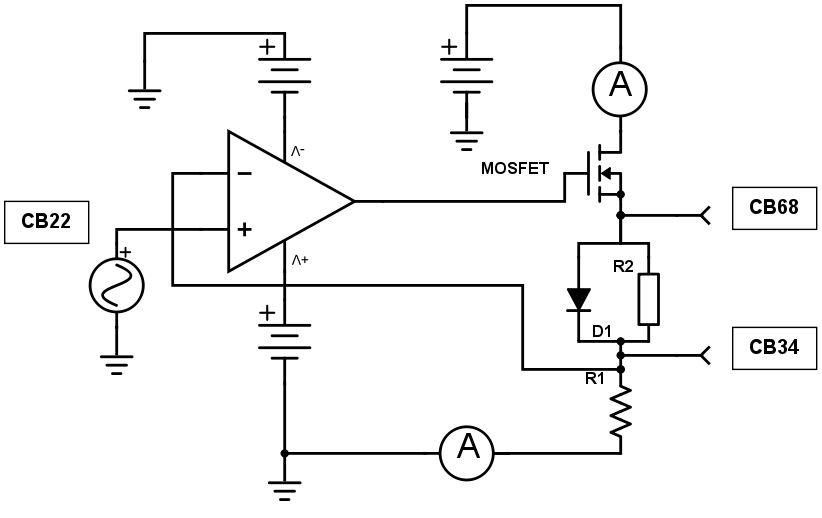
\includegraphics[width=0.7\linewidth]{./WEEK08-ES12}
\caption{Circuito del generatore di corrente: si noti che NON vi è un parallelo fra il LED e la resistenza R2, ma una doppia scelta.}
\label{fig:WEEK08-ES12}
\end{figure}


\subsection{Resistenza}
Scegliamo al posto del laser una resistenza $R_2 = 360(3) \Omega$, di potenza massima $1/2$W per andare sul sicuro, come resistenza $R_1$ scegliamo invece $R_1 = 215(2) \Omega$. L'opamp è alimentato a $V_{CC} = \pm 15V$, e la tensione $V_{in}$ sull'ingresso non invertente è stata scelta minore di 4.5V poichè, per questi valori, si verifica sperimentalmente che la tensione ai capi della resistenza $R_1$ è uguale a quella fornita in ingresso (ipotesi di opamp ideale): ciò viene meno a $V_{in} > 4.5V$ poichè l'opamp entra in regime di saturazione,la tensione in uscita satura a circa 13V e non è più sufficiente a controllare la corrente di drain.\\
Considerando il ramo formato da $R_1$ e $R_2$, questi non sono altro che un partitore di tensione e ciò ci permette di scrivere in maniera agevole la $\Delta V = V_{S} - V_1 = V_{in} \frac{R_2}{R_1} \Rightarrow V_{S} = V_{in} (1 + \frac{R_2}{R_1})$. Queste relazioni sono molto ben verificate e, in particolare, in Figura (\ref{fig:es17_fit}) si riporta il fit di $V_S$ in funzione della $V_{in}$: il coefficiente angolare previsto con le resistenze a nostra disposizione coincide nei limiti dell'errore con quello restituito dal fit.\\
Un risultato analogo lo otteniamo simulando lo stesso circuito con \textsc{tina}, impiegando tutti i componenti opportuni, tra cui anche il \textsc{mosfet bs170} che siamo riusciti a importare dal sito ufficiale della \textit{Fairchild}. I risultati della simulazione con \textsc{tina} sono riportati in Figura (\ref{fig:es_12_oldmosfet_noled_graph}). Notiamo che il coefficiente angolare della relazione evidentemente lineare fra la tensione di \textit{source} e quella di ingresso è di $coeff = 2.64$ perfettamente coincidente con il risultato del best-fit dei dati sperimentali. Anche l'offset a $V_{in} = 0V$, $V_{off} = 5.25 \si{mV}$ è molto prossimo a quello fittato. Vediamo infine che la tensione di source va in saturazione per valori di circa 9.9V, (poichè l'op-amp satura), per cui limitiamo la spazzata di $V_{in}$ fino a valori inferiori a 3.5V. La corrente massima di source, infine, risulta inferiore a 20mA e quindi al di sotto della corrente $I_{F,max} = 30mA$ del LED da noi scelto, motivo per cui possiamo ora provare a sostituirlo alla resistenza $R_2$.\\ 

\begin{figure}
\centering
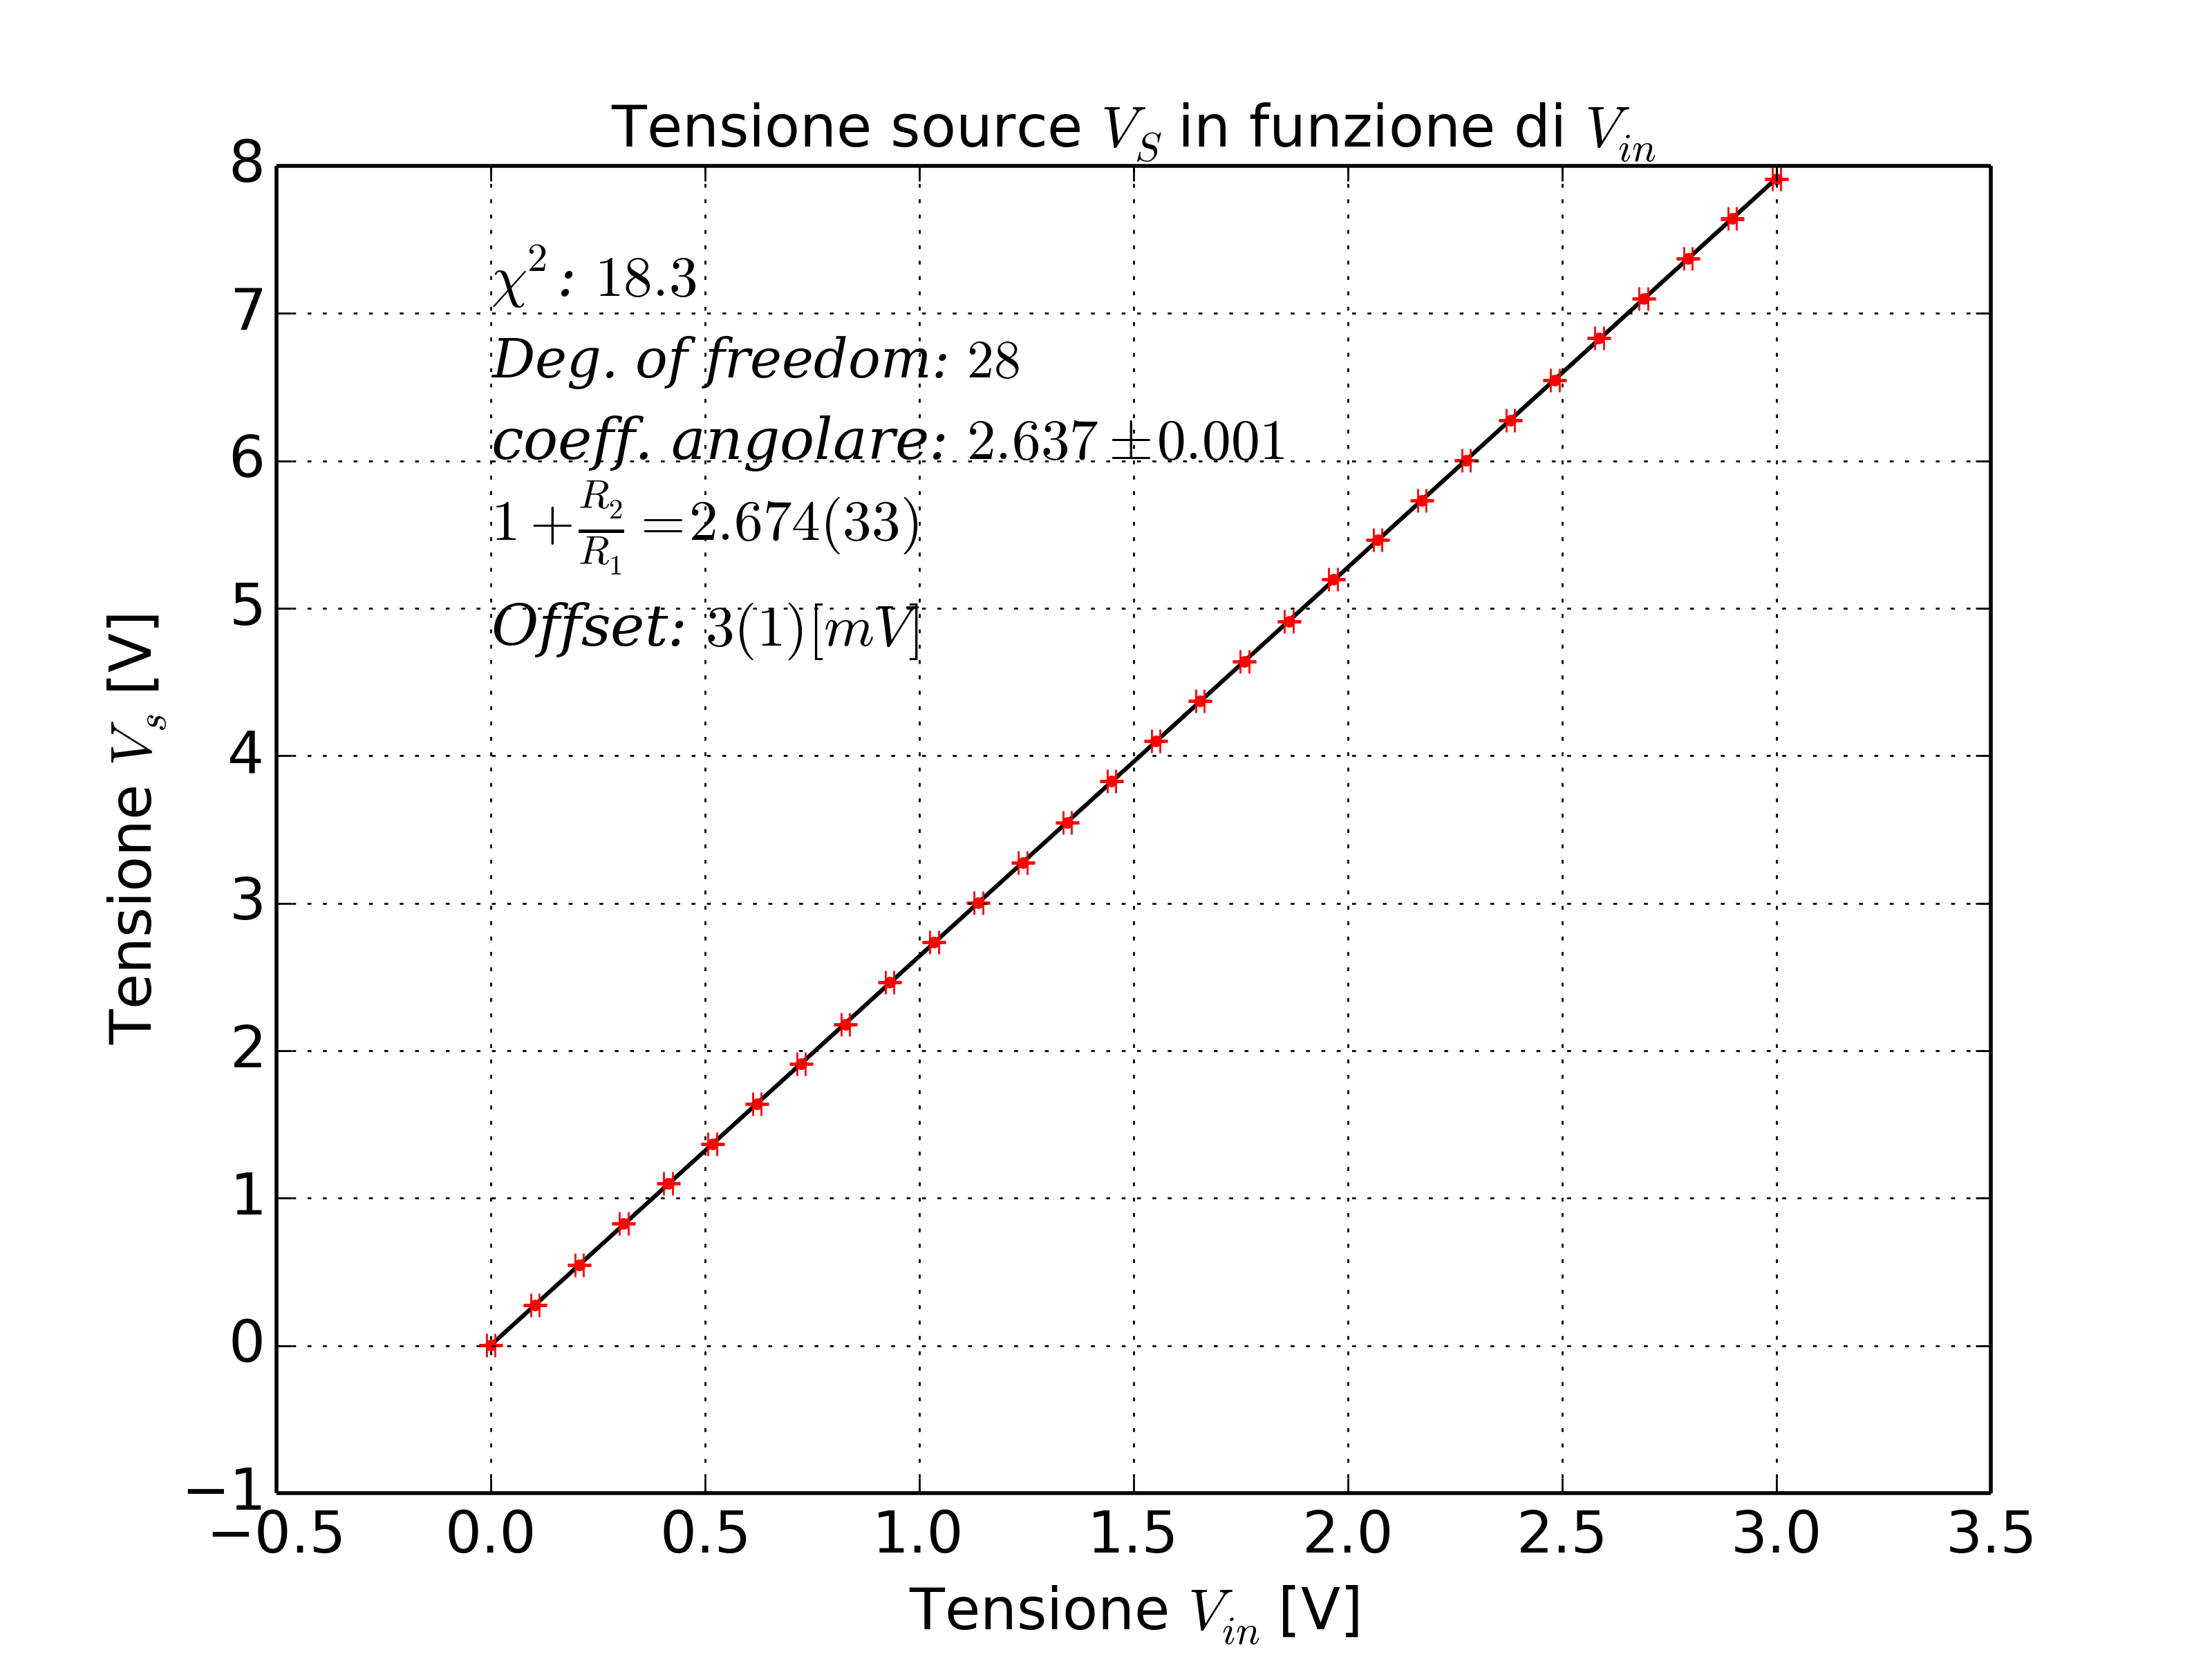
\includegraphics[width=0.9\linewidth]{./es17_fit}
\caption{$V_S$ in funzione di $V_{in}$ - fit della retta.}
\label{fig:es17_fit}
\end{figure}


\begin{figure}
\centering
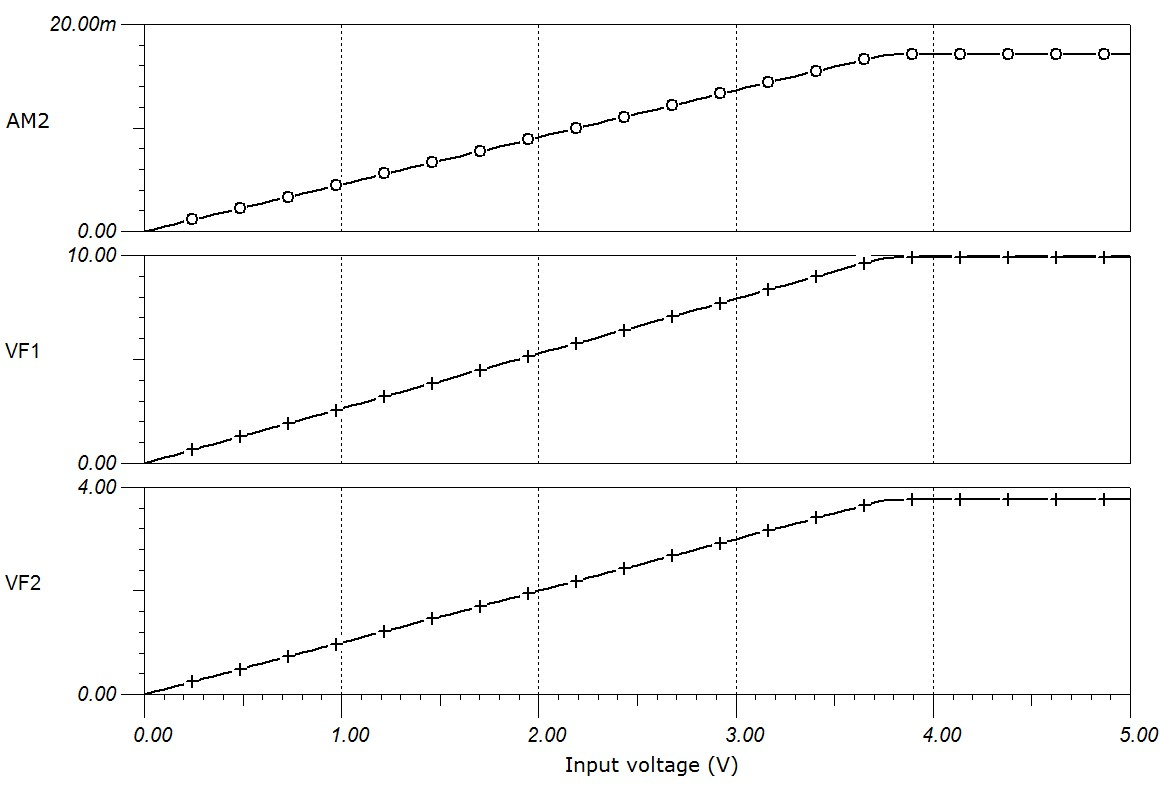
\includegraphics[width=0.8\linewidth]{./es_12_oldmosfet_noled_graph}
\caption{Risultati della simulazione con TINA: corrente di source, tensione di source e tensione sulla resistenza $R_1$ in funzione di $V_{in}$.}
\label{fig:es_12_oldmosfet_noled_graph}
\end{figure}


\subsection{LED}
Ripetiamo ora la stessa procedura impiegando un LED (\textsc{hlmpc115}) al posto della resistenza $R_2$. Riportiamo in Figura (\ref{fig:es18_prova1}) il grafico della tensione dell'anodo $V_a$ in funzione di quella in ingresso. La somiglianza con la caratteristica I-V del LED è notevole (ruotando gli assi, in modo che la $V_{in}$, che è proporzionale alla corrente I, vada sulle ordinate). Per rendercene meglio conto, plottiamo lo stesso grafico in scala bilog, così da evidenziare la funzione esponenziale nella relazione (Figura (\ref{fig:es18_0-2_prova1})).\\
Provando anche questa volta a simulare con \textsc{tina} il comportamento del circuito, non otteniamo però dei risultati in linea con quelli osservati sperimentalmente; infatti la tensione di source sembra aumentare quasi linearmente con la $V_{in}$ e neanche un plot in scala logaritmica sembra evidenziare comportamenti di questo tipo. Ciò potrebbe essere dovuto al fatto che il modello del LED da noi usato (\textsc{hlmpc115}) non esiste nel database di TINA e nè siamo riusciti a trovarlo altrove, motivo per cui è stato impiegato un altro LED che presentasse almeno alcuni parametri simili (come la corrente $I_F$ massima), ma comunque sensibilmente diverso. I risultati della simulazione sono in Figura (\ref{fig:es_12_newmosfet_led_graph}).

\begin{figure}
\centering
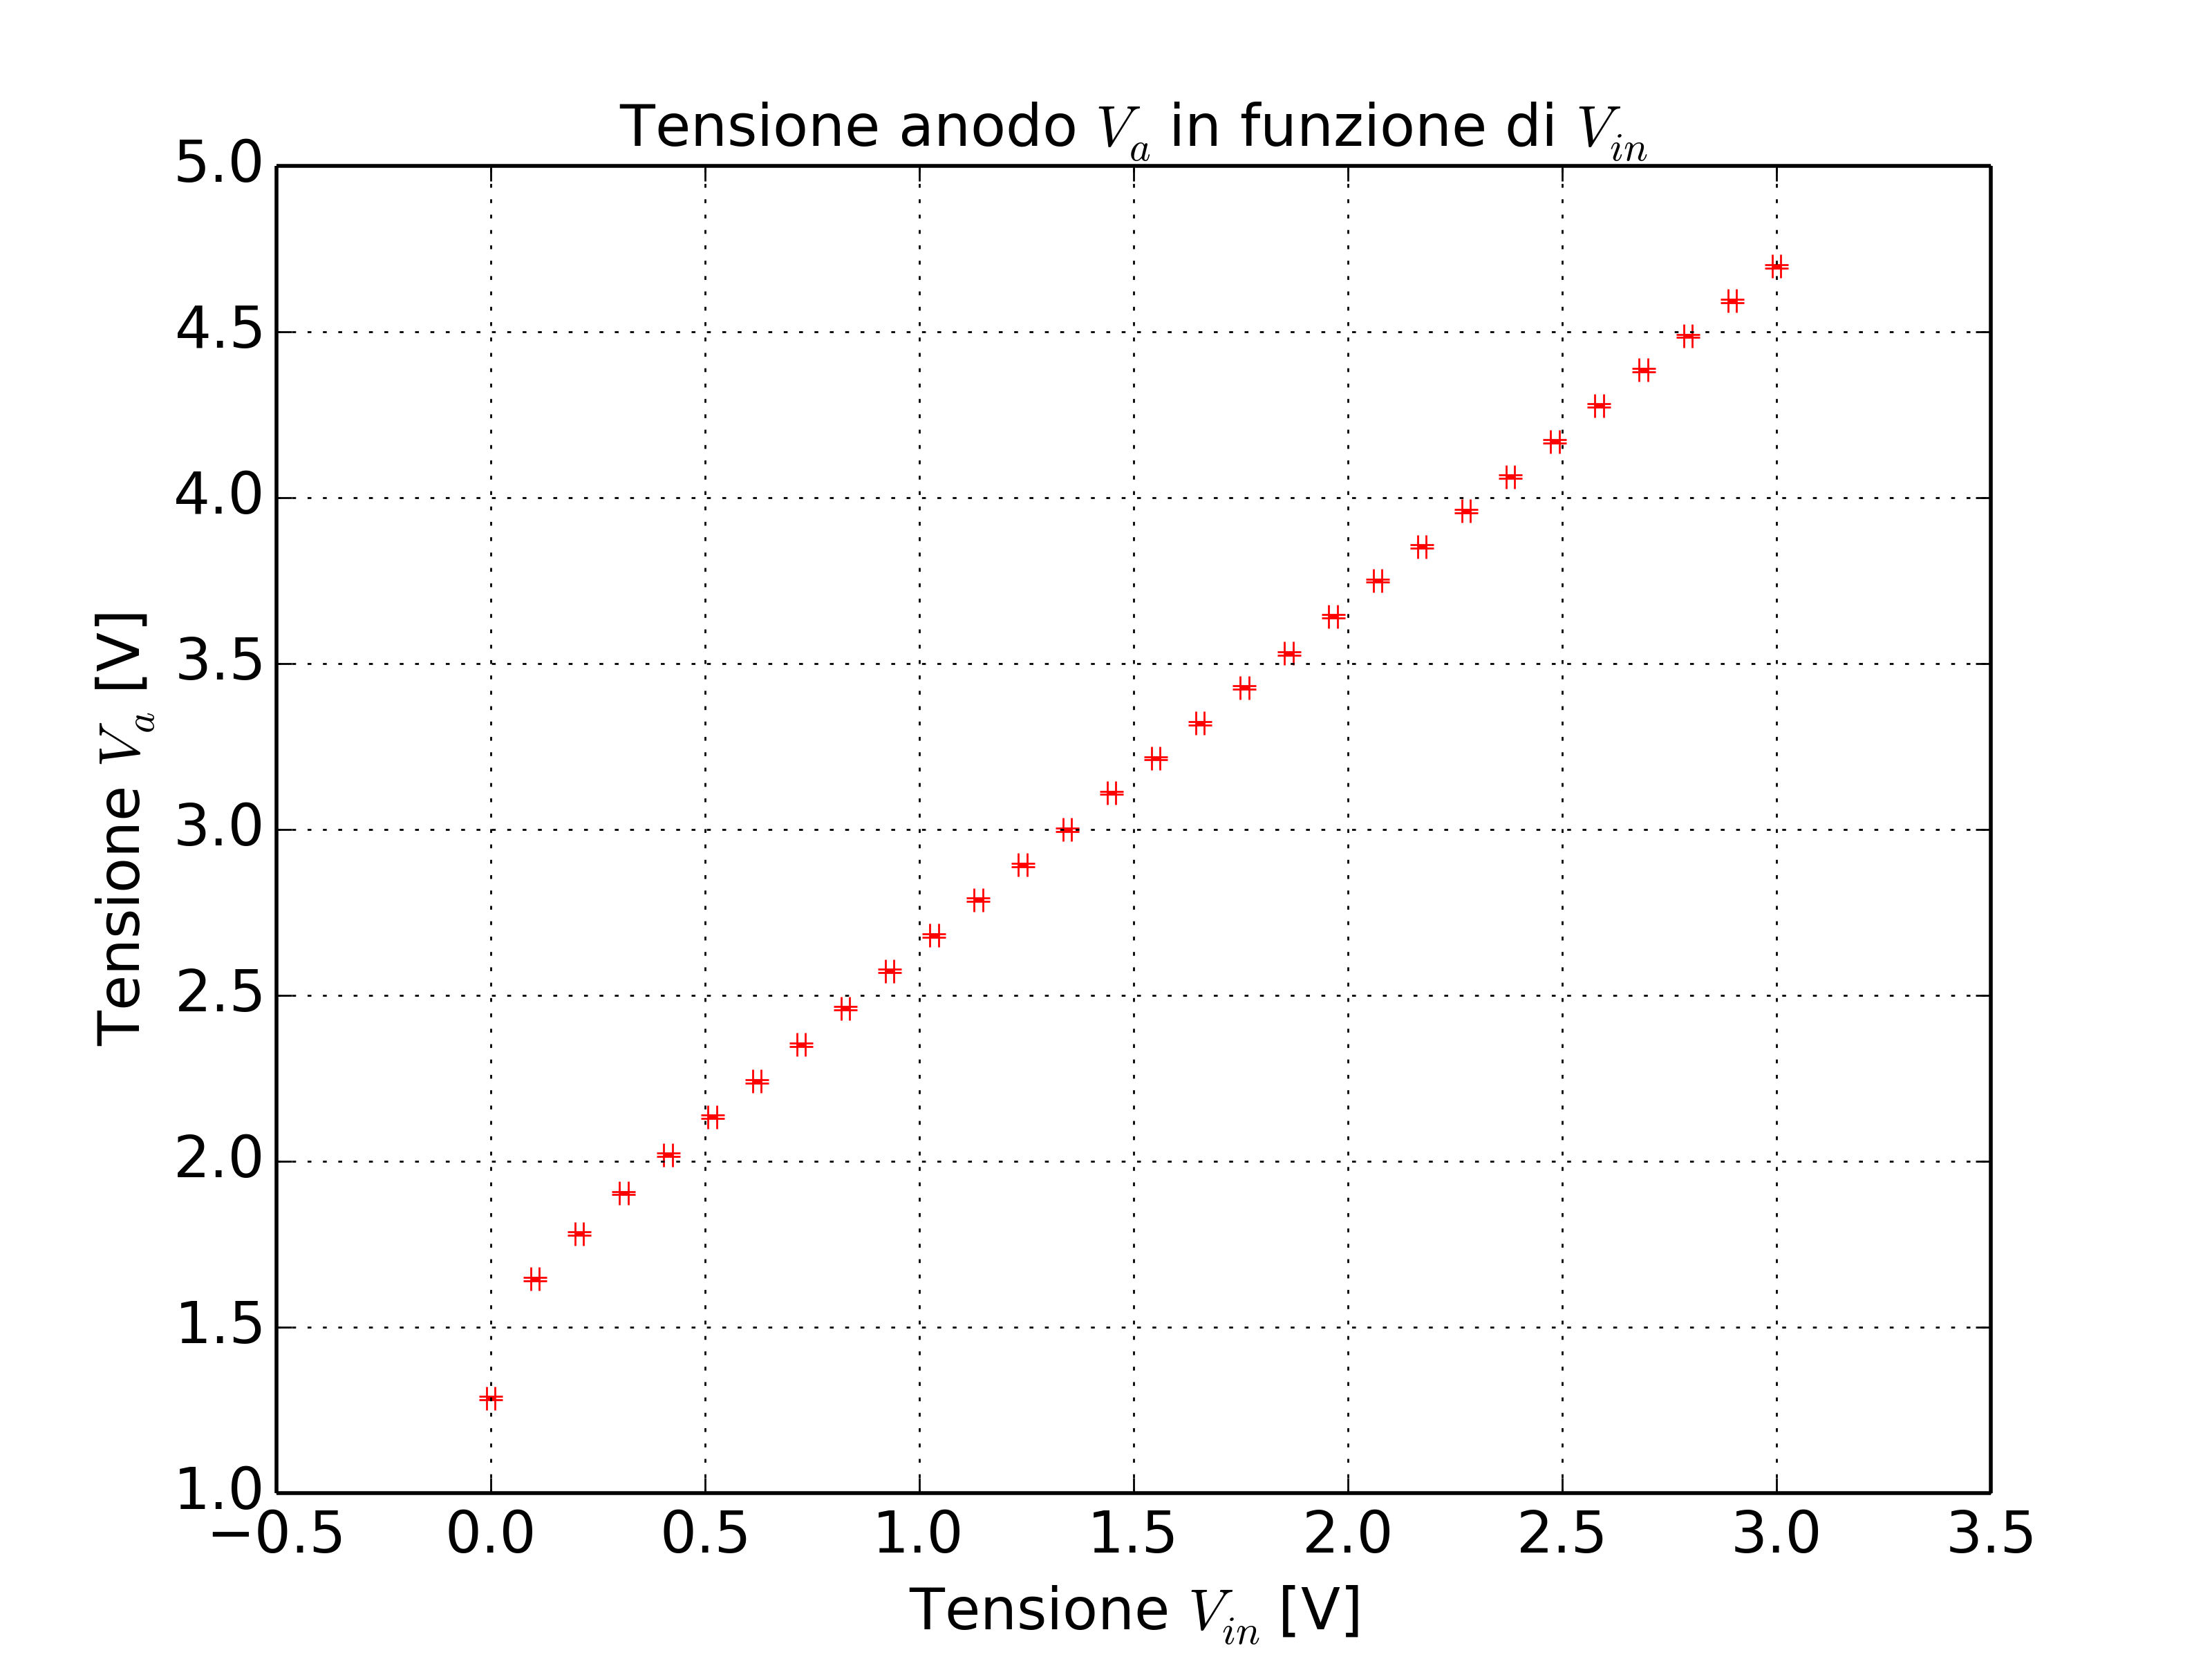
\includegraphics[width=0.9\linewidth]{./es18_prova1}
\caption{Tensione dell'anodo in funzione del segnale in ingresso.}
\label{fig:es18_prova1}
\end{figure}

\begin{figure}
\centering
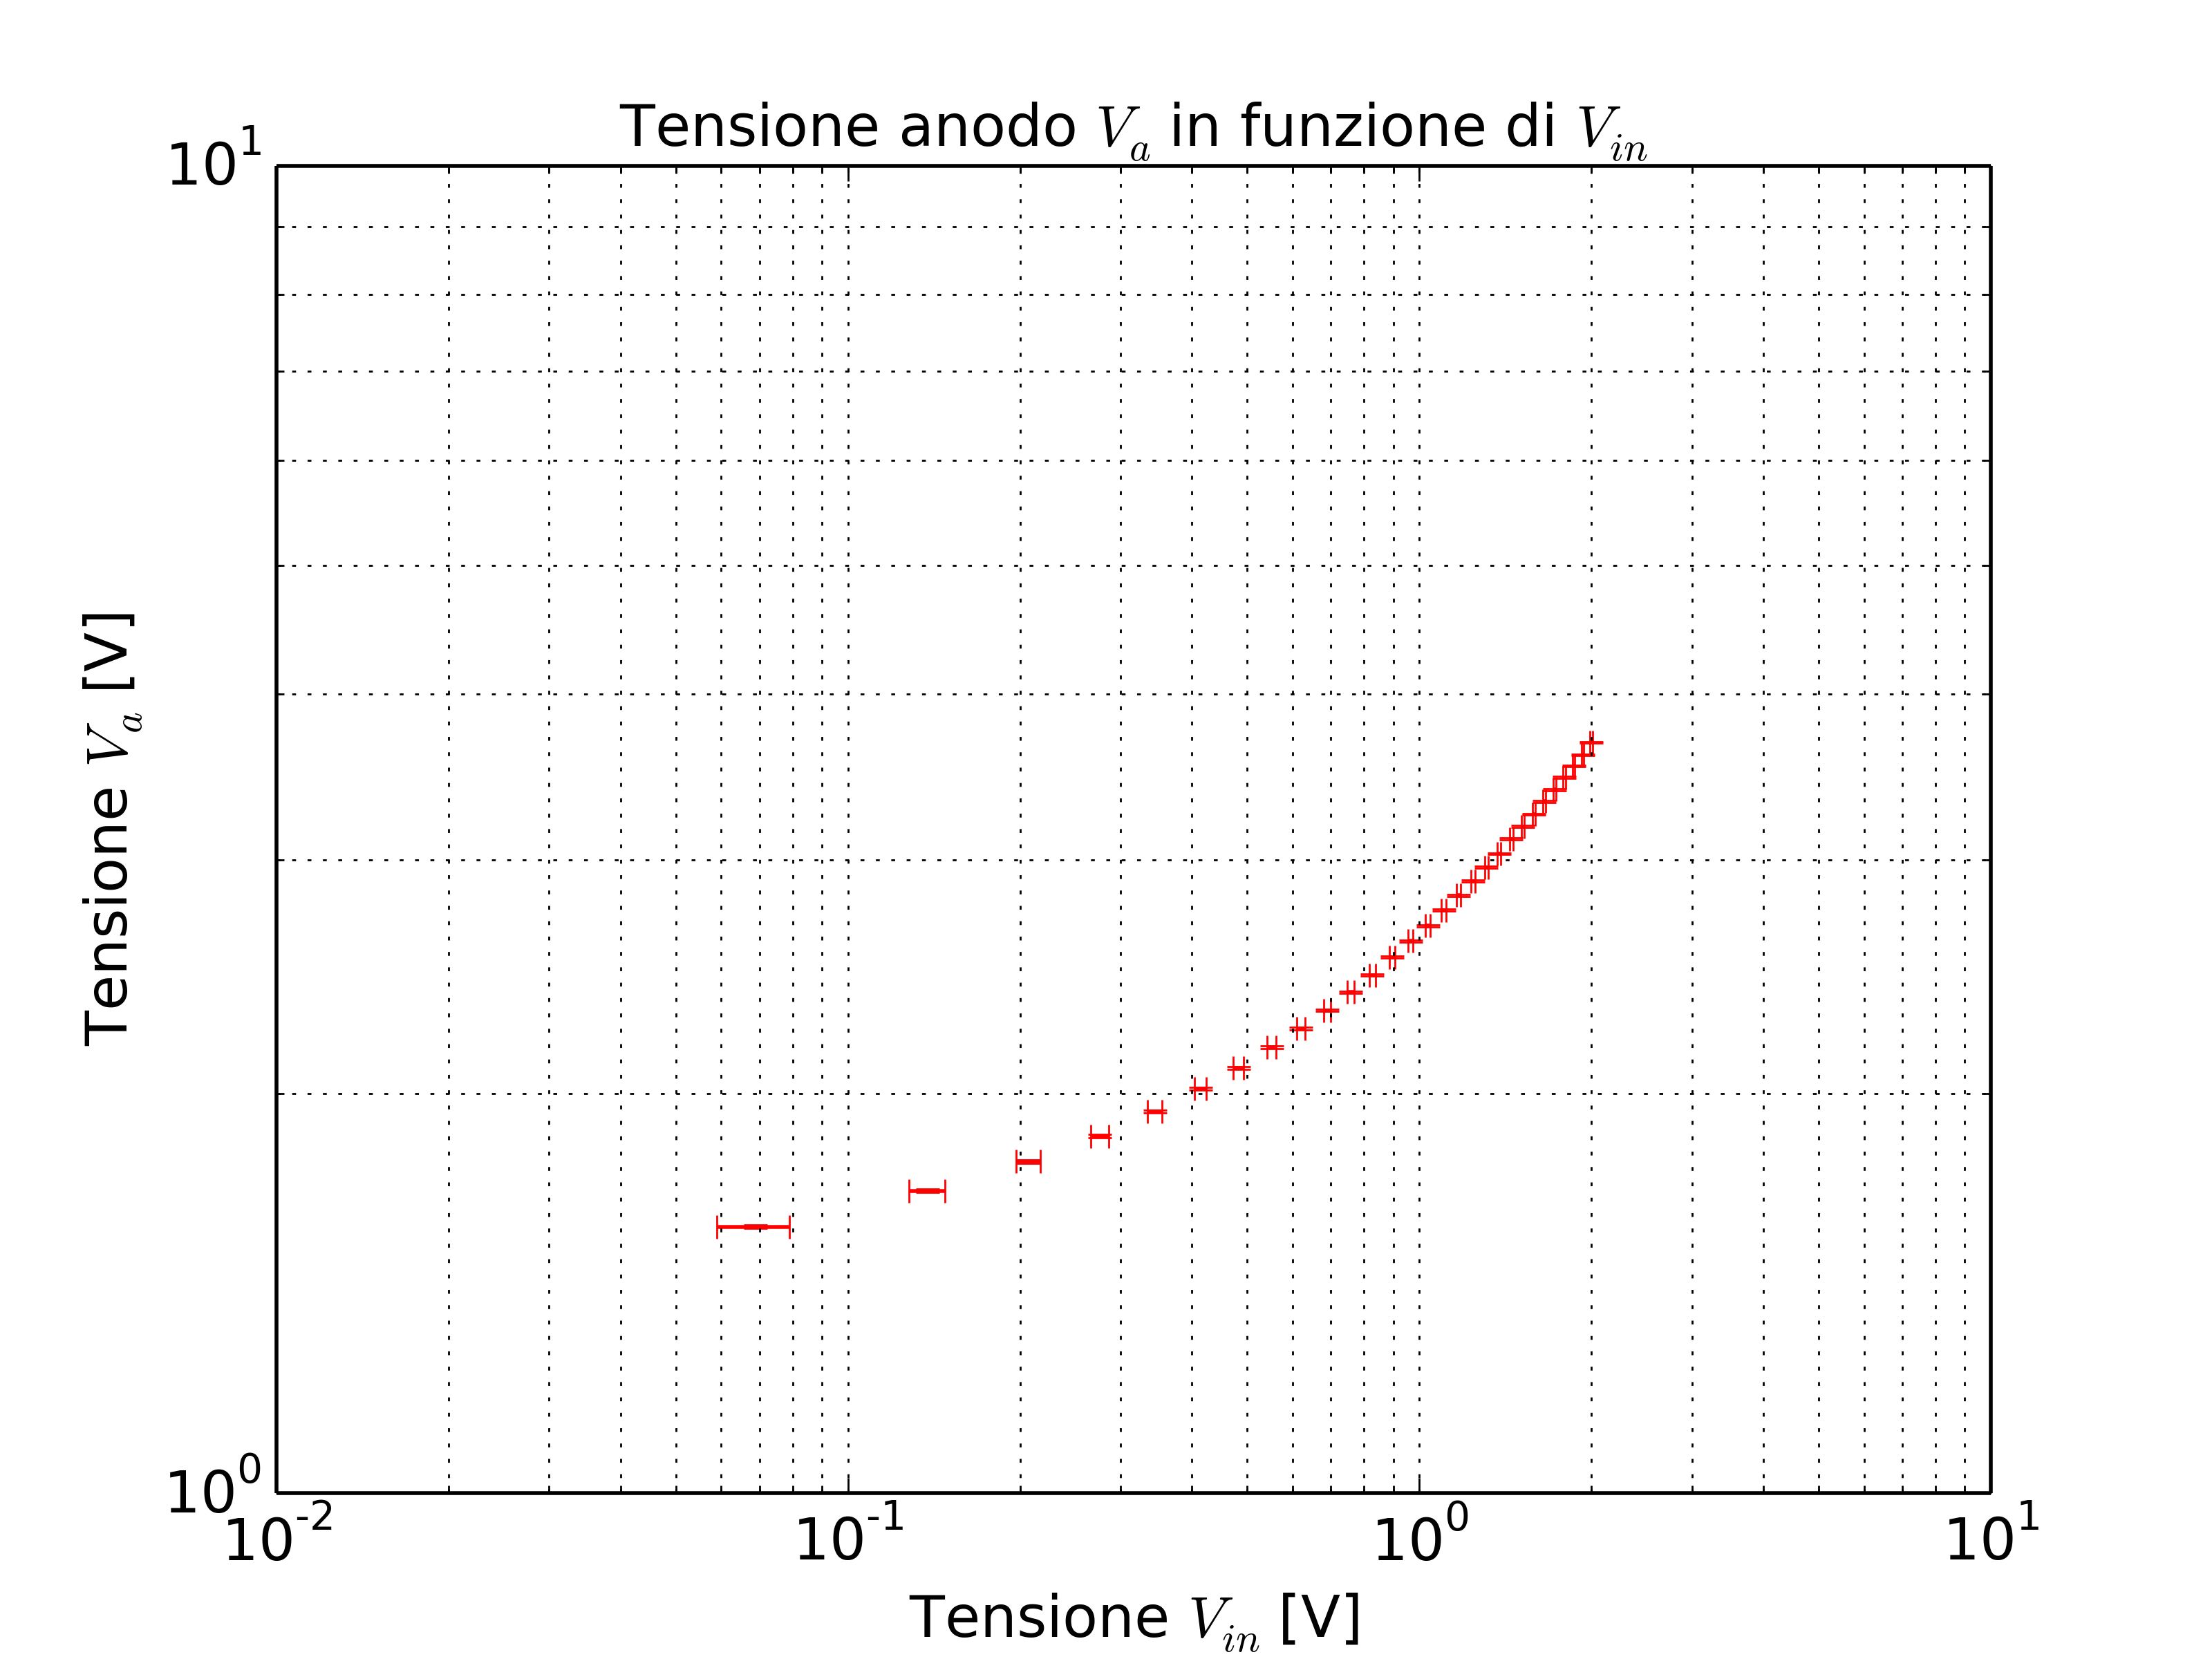
\includegraphics[width=0.9\linewidth]{./es18_0-2_prova1}
\caption{Tensione dell'anodo in funzione del segnale - scala bilog}
\label{fig:es18_0-2_prova1}
\end{figure}

\begin{figure}
\centering
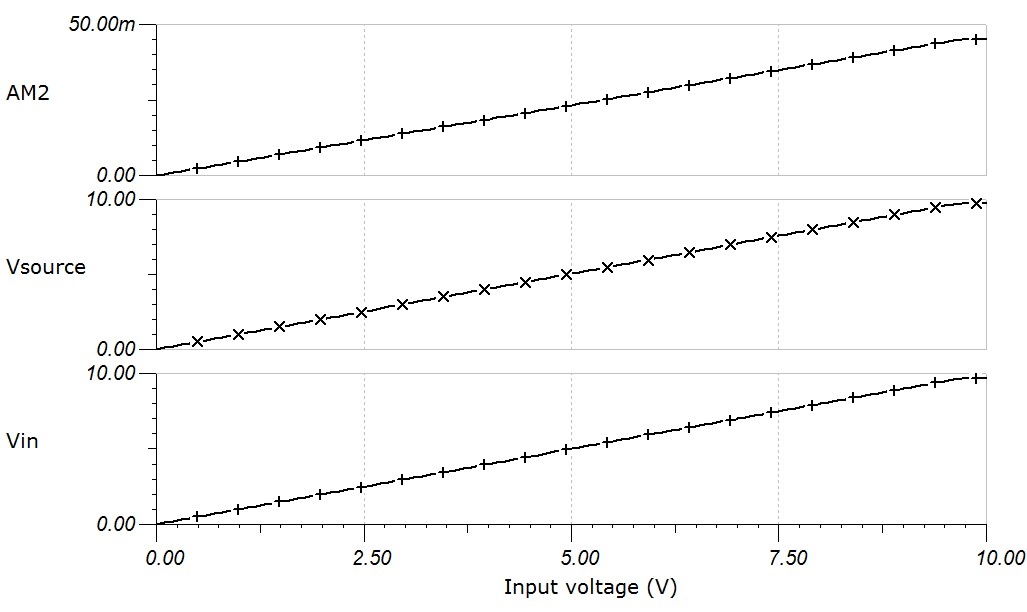
\includegraphics[width=0.8\linewidth]{./es_12_newmosfet_led_graph}
\caption{Risultati della simulazione con TINA: corrente di source, tensione di source e tensione sulla resistenza $R_1$ in funzione di $V_{in}$.}
\label{fig:es_12_newmosfet_led_graph}
\end{figure}


Tramite il VI \textit{Traccia\_I\_V\_DIFF} possiamo direttamente tracciare la curva I-V del LED: il risultato è in Figura (\ref{fig:es19}). La tensione $V_F$ è stata misurata eseguendo la differenza fra il segnale della \textsc{cb68} e quello della \textsc{cb34}; la corrente $I_F$, invece, moltiplicando il valore della resistenza di carico $R_1$ per il segnale della \textsc{cb34}. E' interessante notare come, pur impostando la spazzata su $V_{in}$ partendo da zero, questo non corrisponda ad un valore di $V_F = 0$, ma piuttosto a $V_F \simeq 1.3 V$. Questo potrebbe essere dovuto ad una qualche tensione di \textit{offset} in uscita dall'op-amp prossima alla tensione di soglia del LED, per cui la corrente in uscita da quest'ultimo risulti dell'ordine di pochi $\mu$A (come verificato nelle esperienze precedenti), non rilevabile nella scala del grafico.

\begin{figure}
\centering
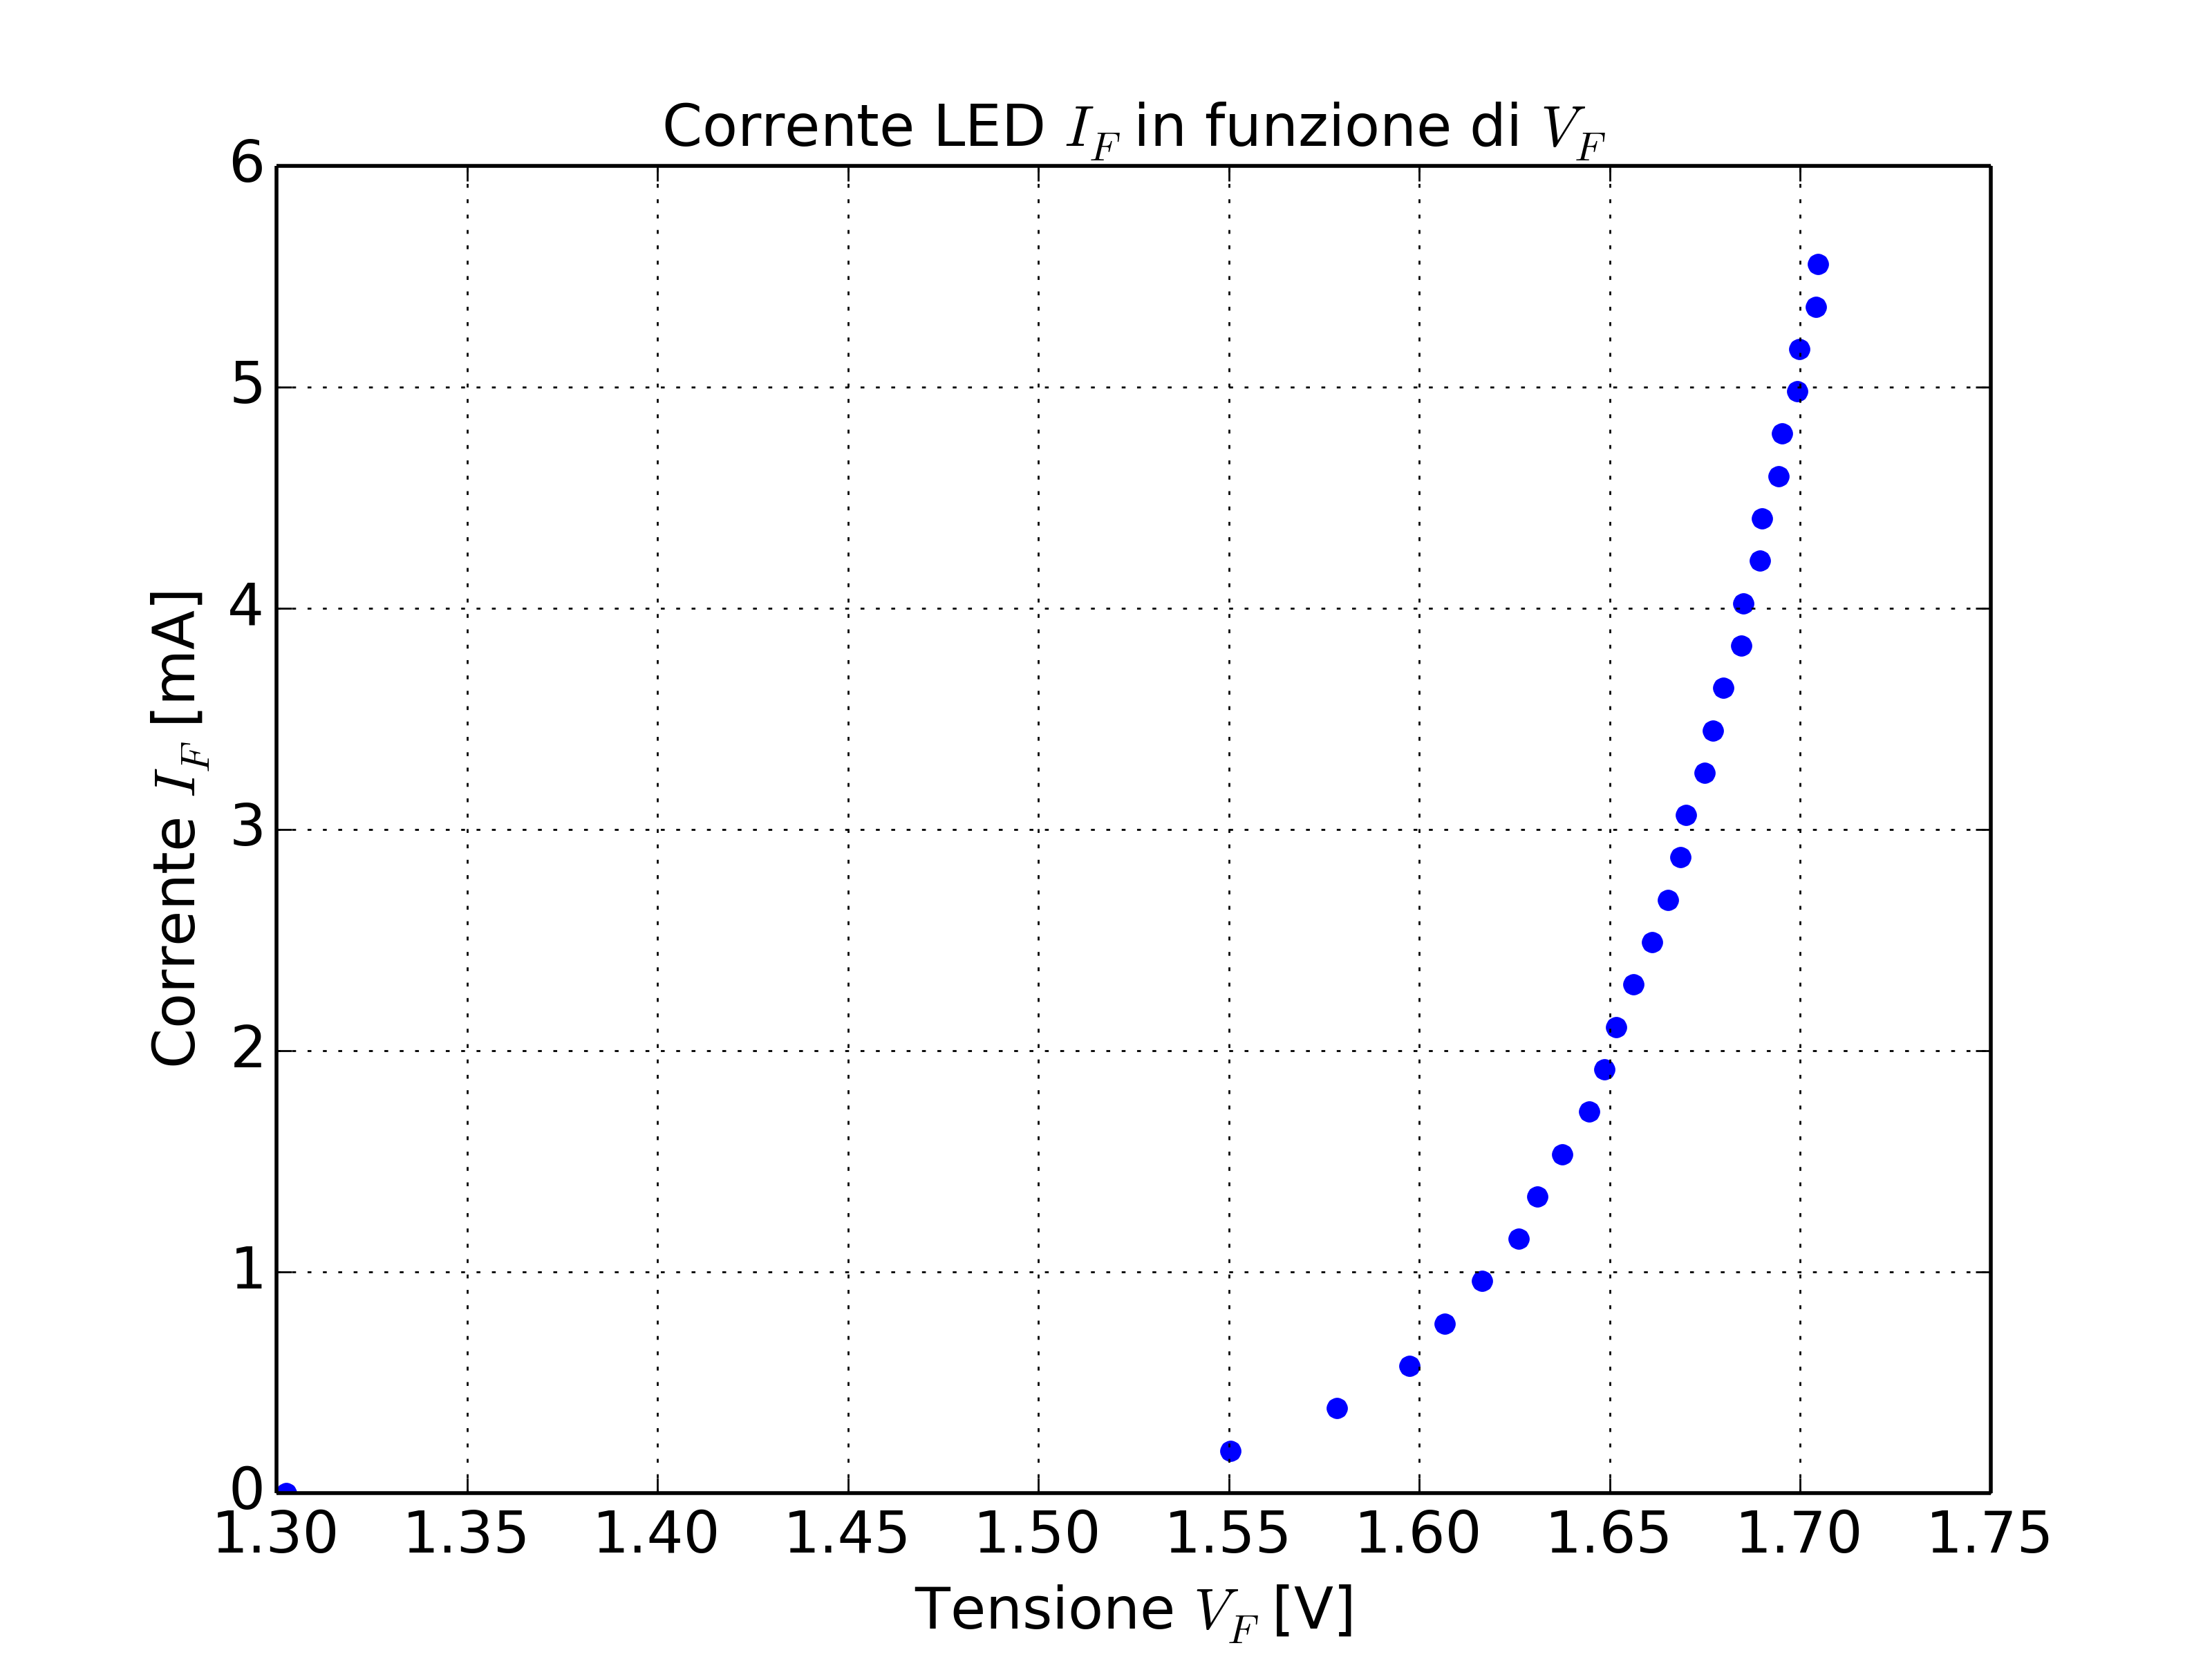
\includegraphics[width=0.9\linewidth]{./es19}
\caption{Caratteristica I-V del LED}
\label{fig:es19}
\end{figure}

A questo punto si può sostituire il LED con il laser a diodo per tracciarne la caratteristica I-V. Tuttavia, per ragioni di tempo, non siamo riusciti ad affrontare questa parte dell'esperienza.


\begin{thebibliography}{5}

	%Each item starts with a \bibitem{reference} command and the details thereafter.
	\bibitem{HOP96} % Transaction paper
	Datasheet, $\mu $A741 General-Purpose Operational Amplifiers. SLOS094E – NOVEMBER 1970  –REVISED JANUARY 2015.
	\url{http://www.ti.com/lit/ds/symlink/ua741.pdf}

	\bibitem{MJ06} % Conference paper
	Product data sheet: 1N4148 High-speed diodes. NXP Semiconductors 2004 Aug 10.
	\url{http://www.nxp.com/documents/data_sheet/1N4148_1N4448.pdf}

	\bibitem{MJH0} % Conference paper
	Product data sheet: AD711 op-amp.
	\url{http://www.analog.com/media/en/technical-documentation/data-sheets/AD711.pdf}
	
	\bibitem{JH06} % Conference paper
	Product data sheet: OP27 op-amp.
	\url{http://www.analog.com/media/en/technical-documentation/data-sheets/OP27.pdf}
	
	\bibitem{JH6} % Conference paper
	Product data sheet: tl081 op-amp.
	\url{http://www.ti.com/lit/ds/symlink/tl081.pdf}

	\bibitem{M06} % Conference paper
	Paul Horowitz, Winfield Hill - The Art of Electronics. Cambridge University Press (1989).
	
\end{thebibliography}

\end{document}